\section{First-Price Auctions II: The Guerre-Perrigne-Vuong Approach}\label{sec:15-gpv}

The direct methods of \cref{sec:15-direct} start from a parametric value distribution and solve for the equilibrium at every trial parameter. \citet{GuerrePerrigneVuong2000}, henceforth GPV, reversed the direction of the argument. They start from the distribution of observed bids and recover the value that rationalizes each bid. No equilibrium is ever computed, and no parametric family is assumed. This section develops their approach in full. It is the template for almost every structural method for first-price auctions that later sections use.

\casehead{The question} GPV pose three questions about the symmetric independent private values (SIPV) model of the first-price auction \citep[p.~526]{GuerrePerrigneVuong2000}. Does the model restrict the distribution of observable bids, so that it can be tested? Does identification of the value distribution require parametric assumptions? Can one estimate the value distribution without parametric assumptions and without solving for the equilibrium? Their answers are yes, no and yes. The model places two testable restrictions on bids. The value distribution is identified nonparametrically and constructively. A two-step kernel estimator recovers it, and no estimator can converge uniformly at a faster rate.

\casehead{Data} The method needs, for each auction $t=1,\dots,T$, all submitted bids $B_{1t},\dots,B_{n_tt}$, the number of bidders $n_t$, and the observed characteristics $Z_t$ of the object. These are the records of a sealed-bid first-price auction, such as a timber sale, a highway procurement or an offshore oil lease sale. GPV illustrate the method on simulated data, and we follow them in \cref{sec:15-gpv-mc}. Applications to field data appear in \cref{sec:15-apv,sec:15-uh,sec:15-als}.

\subsection{Setting and the inversion}\label{sec:15-gpv-insight}

We first state the model and the assumptions on the data-generating process, following GPV, Section 3.1. A single indivisible object is sold in each auction by a first-price sealed-bid auction. The highest bidder wins and pays her bid. Throughout \cref{sec:15-gpv-insight,sec:15-gpv-ident,sec:15-gpv-smooth,sec:15-gpv-estimator,sec:15-gpv-rates,sec:15-gpv-mc} the reserve price does not bind, so every potential bidder submits a bid and $n_t$ is the number of bidders who could have participated. \Cref{sec:15-gpv-reserve} treats a binding reserve price.

Let $Z_t\in\R^d$ collect the continuous characteristics of the object in auction $t$, and let $\mathcal I$ denote the set of possible numbers of bidders. The characteristics $Z_t$ are common knowledge among bidders. Their role is to absorb observed heterogeneity across auctions. They are not instruments.

\begin{assumption}[Sampling, GPV Assumption A1]\label{ass:15-gpv-sampling}
(i) Auctions are independent: the arrays $(Z_t,n_t,V_{1t},\dots,V_{n_tt})$, $t=1,2,\dots$, are independent across $t$, and the vectors $(Z_t,n_t)$ are identically distributed with density $f_{Zn}(z,n)$.
(ii) In each auction $t$, the values $V_{1t},\dots,V_{n_tt}$ are independent and identically distributed conditional on $(Z_t,n_t)$, with distribution $F(\cdot\mid Z_t,n_t)$ and density $f(\cdot\mid Z_t,n_t)$.
\end{assumption}

\begin{assumption}[Regularity, GPV Assumption A2]\label{ass:15-gpv-regularity}
The set $\mathcal I$ is a bounded subset of $\{2,3,\dots\}$, and the following hold.
(i) For each $n\in\mathcal I$, the support of $(V,Z)$ is $\{(v,z):z\in[\underline z,\bar z],\ v\in[\underline v(z),\bar v(z)]\}$ with $\underline z<\bar z$.
(ii) $f(v\mid z,n)\ge c_f>0$ on this support, and $f_{Zn}(z,n)\ge c_f>0$ on the support of $(Z,n)$.
(iii) For each $n\in\mathcal I$, $F(\cdot\mid\cdot,n)$ and $f_{Zn}(\cdot,n)$ have $R+1$ continuous bounded partial derivatives on their supports, with $R\ge 1$.
\end{assumption}

\Cref{ass:15-gpv-sampling} rules out dependence of values across auctions. GPV state part (i) for $(Z_t,n_t)$ only and invoke independence of values across auctions in the text, so we make it explicit. Such dependence would create dynamic incentives that the static equilibrium ignores. It allows the number of bidders to depend on the characteristics of the object. Part (iii) of \cref{ass:15-gpv-regularity} implies that the value density $f(\cdot\mid z,n)$ has $R$ bounded continuous derivatives. The integer $R$ measures smoothness and governs every rate of convergence below. The density is bounded away from zero, which keeps the bid density away from zero as well (\cref{prop:15-gpv-smooth}). GPV also assume, in the spirit of the theory, that $Z_t$ contains everything that bidders know about the object \citep[footnote 11]{GuerrePerrigneVuong2000}. Unobserved heterogeneity is the subject of \cref{sec:15-uh}.

\casehead{Equilibrium} Fix an auction with characteristics $z$ and $n$ bidders, and suppress $(z,n)$ when no confusion arises. Set the reserve price equal to $\underline v$. By \cref{prop:14-rs}, which gives the bid function of \citet{RileySamuelson1981}, the unique symmetric equilibrium bid is
\begin{equation}\label{eq:15-gpv-rs}
\beta(v)=v-\frac{1}{F(v)^{n-1}}\int_{\underline v}^{v}F(u)^{n-1}\,du,
\end{equation}
which is \eqref{eq:14-rs-bid} with $r=\underline v$ (GPV, eqs.~(1) and~(8)). It solves the differential equation
\begin{equation}\label{eq:15-gpv-ode}
1=\big(v-\beta(v)\big)(n-1)\frac{f(v)}{F(v)}\frac{1}{\beta'(v)}
\end{equation}
with the boundary condition $\beta(\underline v)=\underline v$ (GPV, eq.~(2)). This is \eqref{eq:14-rs-ode} divided by $\beta'(v)F(v)^{n-1}$. The bid function is strictly increasing on $[\underline v,\bar v]$.

\casehead{Why identification is not obvious} As \cref{sec:15-fpa-hard} explained, the bid distribution $G$ depends on $F$ in two ways. It depends on $F$ directly, because values are drawn from $F$. It also depends on $F$ through the strategy $\beta$, which by \eqref{eq:15-gpv-rs} is itself a functional of $F$. A direct method must untangle both channels for every trial value of $F$.

\casehead{The inversion} GPV observe that the first-order condition can be written so that the derivative $\beta'$, the distribution $F$ and the density $f$ disappear together. We derive the resulting formula step by step. Let $[\underline b,\bar b]=[\beta(\underline v),\beta(\bar v)]$ denote the support of bids, and note that $\underline b=\underline v$.

\emph{Step 1.} We express the bid distribution through $F$ and $\beta$. For $b\in[\underline b,\bar b]$, the strict monotonicity of $\beta$ gives
\[
G(b)=\Pr(B_i\le b)=\Pr\big(V_i\le\beta^{-1}(b)\big)=F\big(\beta^{-1}(b)\big).
\]

\emph{Step 2.} We differentiate. By the inverse function rule,
\[
g(b)=f\big(\beta^{-1}(b)\big)\frac{d\beta^{-1}(b)}{db}=\frac{f\big(\beta^{-1}(b)\big)}{\beta'\big(\beta^{-1}(b)\big)}.
\]

\emph{Step 3.} We take the ratio. Write $v=\beta^{-1}(b)$. Dividing the result of Step 2 by that of Step 1 gives
\[
\frac{g(b)}{G(b)}=\frac{1}{\beta'(v)}\,\frac{f(v)}{F(v)}.
\]

\emph{Step 4.} We substitute into the equilibrium condition. The right side of Step 3 is exactly the product that appears in \eqref{eq:15-gpv-ode}. Replacing it there and using $\beta(v)=b$ gives
\[
1=(v-b)(n-1)\frac{g(b)}{G(b)}.
\]

\emph{Step 5.} We solve for the value. Dividing by $(n-1)\frac{g(b)}{G(b)}$ and adding $b$ to both sides yields
\begin{equation}\label{eq:15-gpv-xi}
v=\xi(b;G,n)\equiv b+\frac{1}{n-1}\,\frac{G(b)}{g(b)}.
\end{equation}
This is GPV's equation~(3), and it coincides with \eqref{eq:14-foc-G}. With covariates, $G$ and $g$ are replaced by $G(\cdot\mid z,n)$ and $g(\cdot\mid z,n)$ (GPV, eq.~(9)).

Equation \eqref{eq:15-gpv-xi} expresses each value through the bid, the bid distribution, the bid density and the number of bidders. All four are observable or estimable. If bids are equilibrium bids, the value behind each bid must satisfy \eqref{eq:15-gpv-xi}. We call $\xi(\cdot;G,n)$ the \emph{inverse bid function}. In equilibrium it equals $\beta^{-1}$, and it has been obtained without solving \eqref{eq:15-gpv-ode}. We use the symbol $\xi$ for this object throughout the chapter, as GPV do (\cref{tab:15-notation}).

The same equation follows from the bidder's problem written in terms of bids, which is how \cref{sec:14-fpa-G} derived \eqref{eq:14-foc-G}. A bidder with value $v$ facing rivals whose bids are i.i.d.\ with distribution $G$ maximizes $(v-b)G(b)^{n-1}$. The first-order condition rearranges to \eqref{eq:15-gpv-xi}. The derivation above shows that the two routes agree. It also shows why the bid-based form is the right one for identification: it contains only objects that the data reveal.

\casehead{The markdown} The term $\frac{G(b)}{(n-1)g(b)}=v-b$ is the bidder's \emph{markdown}, the shading of the bid below the value. By \eqref{eq:14-markdown}, the relative markdown $\frac{v-b}{b}$ equals the inverse of the elasticity of the win probability $G(b)^{n-1}$ with respect to the bid. A bidder is a monopsonist facing the residual supply curve traced out by the highest rival bid. Equation \eqref{eq:15-gpv-xi} makes the oligopoly analogy of \cref{sec:15-fpa-hard} exact. The distribution of rival bids plays the role of the demand system, and the econometrician observes it directly.

\casehead{Credit and precursors} The idea first appeared in print in \citet{LaffontVuong1993}, who attribute it to an early draft of GPV \citep[Section 3.1]{AtheyHaile2007}. Similar formulas appear earlier in decision-theoretic models of bidding, starting with \citet{Friedman1956}. There each bidder optimizes against an exogenous distribution of rival bids, so the value distribution and the bid distribution need not be linked by $F=G\circ\beta$ \citep[footnote 3]{GuerrePerrigneVuong2000}. In \eqref{eq:15-gpv-xi} the link holds because bidders' beliefs about rival bids are correct in equilibrium.

\subsection{Identification and testable restrictions}\label{sec:15-gpv-ident}

We now state GPV's identification theorem. Let $\mathcal P$ denote the set of distributions on $\R_+$ that are absolutely continuous with an interval support. The support of a distribution in $\mathcal P$ is the closure of the set where its density is positive, so every member of $\mathcal P$ is strictly increasing on its support \citep[footnote 4]{GuerrePerrigneVuong2000}. Let $\mathbf G$ denote the joint distribution of the $n$ bids $(B_1,\dots,B_n)$ in an auction. As in GPV, we restrict attention to strictly increasing and differentiable equilibrium strategies.

\begin{theorem}[\citealp{GuerrePerrigneVuong2000}, Theorem 1]\label{thm:15-gpv-ident}
Let $n\ge 2$, and let $\mathbf G$ belong to $\mathcal P^n$ with support $[\underline b,\bar b]^n$. Consider a first-price sealed-bid auction with symmetric independent private values and a nonbinding reserve price. There exists a value distribution $F\in\mathcal P$ whose equilibrium bids have joint distribution $\mathbf G$ if and only if the following two conditions hold.
\begin{itemize}
\item[(C1)] $\mathbf G(b_1,\dots,b_n)=\prod_{i=1}^n G(b_i)$ for some distribution $G$.
\item[(C2)] The function $\xi(\cdot;G,n)$ defined in \eqref{eq:15-gpv-xi} is strictly increasing on $[\underline b,\bar b]$, and its inverse is differentiable on $[\underline v,\bar v]\equiv[\xi(\underline b;G,n),\xi(\bar b;G,n)]$.
\end{itemize}
When such an $F$ exists, it is unique, its support is $[\underline v,\bar v]$, and
\begin{equation}\label{eq:15-gpv-F}
F(v)=G\big(\xi^{-1}(v;G,n)\big)\qquad\text{for all }v\in[\underline v,\bar v].
\end{equation}
Moreover, $\xi(\cdot;G,n)$ is the inverse of the equilibrium strategy: $\xi(b;G,n)=\beta^{-1}(b)$ for all $b\in[\underline b,\bar b]$.
\end{theorem}

\begin{proof}
We follow GPV, Appendix A.1, and add the global optimality argument that their footnote~5 assumes. Write $\xi(b)$ for $\xi(b;G,n)$.

\emph{Necessity of (C1).} Suppose $F\in\mathcal P$ with support $[\underline v,\bar v]$ rationalizes $\mathbf G$, and let $\beta$ be the equilibrium strategy. Each bid is $B_i=\beta(V_i)$, a fixed function of an independent draw from $F$. Hence the bids are i.i.d., and (C1) holds with $G(b)=F(\beta^{-1}(b))$.

\emph{Necessity of (C2).} The strategy $\beta$ solves \eqref{eq:15-gpv-ode}. Steps 1 to 5 of \cref{sec:15-gpv-insight} show that \eqref{eq:15-gpv-ode} implies $\xi(\beta(v))=v$ for every $v\in[\underline v,\bar v]$. Setting $b=\beta(v)$ gives $\xi(b)=\beta^{-1}(b)$ on $[\underline b,\bar b]$. The inverse of a strictly increasing function is strictly increasing, so $\xi$ is strictly increasing. Its inverse is $\beta$, which is differentiable on $[\underline v,\bar v]=[\xi(\underline b),\xi(\bar b)]$. Hence (C2) holds.

\emph{Sufficiency, Step 1: the lower boundary.} Assume (C1) and (C2). We show that
\begin{equation}\label{eq:15-gpv-A1}
\lim_{b\downarrow\underline b}\xi(b)=\underline b.
\end{equation}
Since $\xi$ is strictly increasing, the limit exists. Since $\frac{G}{g}\ge0$, we have $\xi(b)\ge b$, so the limit equals $\underline b+c$ for some $c\ge0$. Suppose that $c>0$. By \eqref{eq:15-gpv-xi},
\[
\frac{G(b)}{g(b)}=(n-1)\big(\xi(b)-b\big)\longrightarrow(n-1)c>0\qquad\text{as }b\downarrow\underline b.
\]
Hence there is $\delta>0$ with $\frac{g(b)}{G(b)}\le\frac{2}{(n-1)c}$ on $(\underline b,\underline b+\delta)$. Because $\frac{d}{db}\ln G(b)=\frac{g(b)}{G(b)}$, integrating over $[b,\underline b+\delta]$ gives
\[
\ln G(b)\ge\ln G(\underline b+\delta)-\frac{2\delta}{(n-1)c}\qquad\text{for all }b\in(\underline b,\underline b+\delta).
\]
The right side is a finite constant, yet $\ln G(b)\to-\infty$ as $b\downarrow\underline b$ because $G(\underline b)=0$. This contradiction shows that $c=0$.

\emph{Sufficiency, Step 2: a candidate distribution.} Set $\underline v=\xi(\underline b)=\underline b$, using \eqref{eq:15-gpv-A1}, and $\bar v=\xi(\bar b)$. Define $F$ on $[\underline v,\bar v]$ by \eqref{eq:15-gpv-F}. By (C2), $\xi^{-1}$ is strictly increasing and differentiable. Since $G$ is strictly increasing on $[\underline b,\bar b]$ and absolutely continuous, $F$ is strictly increasing and absolutely continuous, with $F(\underline v)=G(\underline b)=0$ and $F(\bar v)=G(\bar b)=1$. Hence $F\in\mathcal P$ with support $[\underline v,\bar v]$.

\emph{Sufficiency, Step 3: the candidate strategy solves the equilibrium equation.} Let $s=\xi^{-1}$. By Step 1, $s(\underline v)=\underline v$. By construction $F(v)=G(s(v))$, so $f(v)=g(s(v))s'(v)$ and
\[
\frac{f(v)}{F(v)}=s'(v)\,\frac{g\big(s(v)\big)}{G\big(s(v)\big)}.
\]
Evaluating \eqref{eq:15-gpv-xi} at $b=s(v)$ gives $v=s(v)+\frac{G(s(v))}{(n-1)g(s(v))}$, which rearranges to
\[
1=\big(v-s(v)\big)(n-1)\frac{g\big(s(v)\big)}{G\big(s(v)\big)}=\big(v-s(v)\big)(n-1)\frac{f(v)}{F(v)}\frac{1}{s'(v)}.
\]
This is \eqref{eq:15-gpv-ode} with the boundary condition $s(\underline v)=\underline v$. By Step 5 of the proof of \cref{prop:14-rs}, its unique solution is the bid function \eqref{eq:15-gpv-rs} associated with $F$. Hence $s=\beta$.

\emph{Sufficiency, Step 4: the candidate strategy is a best response.} Suppose the rivals use $s$ and draw values from $F$. Each rival bid then has distribution $F(s^{-1}(b))=F(\xi(b))=G(b)$. A bidder with value $v$ who bids $b\in[\underline b,\bar b]$ earns $(v-b)G(b)^{n-1}$. Its derivative is
\[
\frac{d}{db}\Big[(v-b)G(b)^{n-1}\Big]=G(b)^{n-2}\Big[(n-1)g(b)(v-b)-G(b)\Big]=(n-1)g(b)G(b)^{n-2}\big[v-\xi(b)\big].
\]
By (C2) the bracket is positive for $b<s(v)$ and negative for $b>s(v)$. The payoff therefore rises up to $b=s(v)$ and falls after it, so $s(v)$ is the best bid in $[\underline b,\bar b]$. A bid above $\bar b$ wins with certainty, like $\bar b$, but costs more. A bid below $\underline b$ never wins and earns zero, which is at most $(v-s(v))G(s(v))^{n-1}\ge0$. Hence $s$ is a symmetric equilibrium. The resulting joint distribution of bids is $\prod_iG(b_i)=\mathbf G$ by (C1).

\emph{Uniqueness.} The necessity part shows that any rationalizing $F$ has an equilibrium strategy with $\beta=\xi^{-1}$. Then $F(v)=G(\beta(v))=G(\xi^{-1}(v))$, which is \eqref{eq:15-gpv-F}. The right side depends only on $G$ and $n$, so $F$ is unique. Its support is $[\xi(\underline b),\xi(\bar b)]=[\underline b,\xi(\bar b)]$ by \eqref{eq:15-gpv-A1}.
\end{proof}

Step 4 of the proof shows the role of (C2) beyond invertibility. The derivative of the payoff factors into a positive term and the gap $v-\xi(b)$. Monotonicity of $\xi$ is exactly the condition under which the first-order condition picks the global maximum. GPV assume second-order conditions in their footnote~5. In the SIPV model (C2) delivers them. \Citet[Section 5.1]{AtheyHaile2007} use the same single-crossing logic for the affiliated private values model with independence or symmetry (\cref{thm:15-ah-rational} below).

\begin{remark}[An equivalent form of (C2)]\label{rem:15-c2}
Suppose $g$ is differentiable on $(\underline b,\bar b)$. Differentiating \eqref{eq:15-gpv-xi} by the quotient rule gives
\[
\xi'(b)=1+\frac{1}{n-1}\,\frac{g(b)^2-G(b)g'(b)}{g(b)^2}=\frac{n}{n-1}-\frac{1}{n-1}\,\frac{G(b)g'(b)}{g(b)^2}.
\]
The derivative of $\frac{g}{G^n}$ is
\[
\frac{d}{db}\frac{g(b)}{G(b)^n}=\frac{g'(b)G(b)^n-nG(b)^{n-1}g(b)^2}{G(b)^{2n}}=\frac{G(b)g'(b)-ng(b)^2}{G(b)^{n+1}}.
\]
Comparing the two displays,
\[
\xi'(b)=-\frac{G(b)^{n+1}}{(n-1)g(b)^2}\,\frac{d}{db}\frac{g(b)}{G(b)^n}.
\]
The factor in front is negative, so $\xi$ is strictly increasing if and only if $\frac{g}{G^n}$ is strictly decreasing \citep[footnote 6]{GuerrePerrigneVuong2000}. A sufficient condition is that $G$ is \emph{log-concave}, that is, $\frac{g}{G}$ is decreasing. Indeed $\frac{g}{G^n}=\frac{g}{G}\cdot G^{-(n-1)}$ is then the product of a positive decreasing function and a positive strictly decreasing function. GPV state this sufficient condition on p.~530. Log-concavity is a property of the bid data, so it can be checked directly.
\end{remark}

Condition (C2) has content. Bid distributions with deep U-shaped densities can violate it, and so can some sharply peaked multimodal densities \citep[p.~530]{GuerrePerrigneVuong2000}. The next example, due to GPV, makes the point concrete.

\begin{example}[Bids that no value distribution rationalizes]\label{ex:15-gpv-counter}
Let $n=2$ and let bids be i.i.d.\ with distribution
\[
G(b)=\Big(\frac{b}{5-4b}\Big)^{\frac15},\qquad b\in[0,1].
\]
This is a valid distribution: $G(0)=0$, $G(1)=1$, and $\frac{b}{5-4b}$ is strictly increasing. We compute the inverse bid function in four steps. First, take logarithms:
\[
\ln G(b)=\frac15\Big[\ln b-\ln(5-4b)\Big].
\]
Second, differentiate:
\[
\frac{g(b)}{G(b)}=\frac15\Big[\frac1b+\frac{4}{5-4b}\Big]=\frac15\cdot\frac{5-4b+4b}{b(5-4b)}=\frac{1}{b(5-4b)}.
\]
Third, substitute into \eqref{eq:15-gpv-xi} with $n-1=1$:
\[
\xi(b)=b+b(5-4b)=6b-4b^2.
\]
Fourth, differentiate: $\xi'(b)=6-8b$, which is negative for $b>\frac34$. Condition (C2) fails. The implied value peaks at $\xi(\frac34)=\frac94$ and falls to $\xi(1)=2$. A bidder who bids $0.9$ would need a lower value, $2.16$, than a bidder who bids $0.8$, whose implied value is $2.24$. Both cannot be best responses to the same distribution of rival bids, so no value distribution generates these bids in equilibrium.

The density behind this example is U-shaped. Multiplying the second step by $G$ gives $g(b)=b^{-\frac45}(5-4b)^{-\frac65}$. Its logarithmic derivative is $-\frac{4}{5b}+\frac{24}{5(5-4b)}$, which vanishes at $b=\frac12$. The density falls from infinity at $b=0$ to $g(\frac12)\approx0.47$ and rises to $g(1)=1$. The mass of high bids is too thin relative to the mass just below them. Consistently with \cref{rem:15-c2}, the function $\frac{g}{G^2}=b^{-\frac65}(5-4b)^{-\frac45}$ falls on $(0,\frac34)$ and rises on $(\frac34,1)$.

For contrast, let bids be uniform on $[0,1]$ with $n=2$. Then $\frac{G}{g}=b$ and $\xi(b)=2b$, which is strictly increasing. Formula \eqref{eq:15-gpv-F} gives $F(v)=G(\frac v2)=\frac v2$ on $[0,2]$. These bids come from values uniform on $[0,2]$, with $\beta(v)=\frac v2$, as \cref{ex:14-uniform} confirms after rescaling.
\end{example}

The exponent $\frac15$ matters. With exponent $\frac32$ instead, the second step gives $\frac{G}{g}=\frac{b(5-4b)}{7.5}$ and $\xi'(b)=1+\frac{5-8b}{7.5}\ge1-\frac{3}{7.5}>0$, so (C2) would hold. \Cref{fig:15-gpv-counter} plots both bid densities and both inverse bid functions of the example.

\begin{figure}[htbp]
\centering
\begin{subfigure}[t]{0.48\textwidth}
\centering
\begin{tikzpicture}
\begin{axis}[width=0.95\textwidth,height=0.8\textwidth,xmin=0,xmax=1,ymin=0,ymax=2.5,
  xlabel={Bid $b$},ylabel={Bid density $g(b)$},axis lines=left,
  xtick={0,0.25,0.5,0.75,1},xticklabels={$0$,$\frac14$,$\frac12$,$\frac34$,$1$},
  ytick={0,0.5,1,1.5,2,2.5}]
\addplot[thick,blue!70!black,domain=0.03:1,samples=300] {x^(-0.8)*(5-4*x)^(-1.2)};
\addplot[thick,black,dashed,domain=0:1] {1};
\node[font=\small,blue!70!black,align=left,anchor=west] at (axis cs:0.12,1.85) {$g(b)=b^{-\frac45}(5-4b)^{-\frac65}$};
\node[font=\small,anchor=south] at (axis cs:0.5,1.02) {uniform bids, $g(b)=1$};
\end{axis}
\end{tikzpicture}
\caption{Bid densities}
\end{subfigure}\hfill
\begin{subfigure}[t]{0.48\textwidth}
\centering
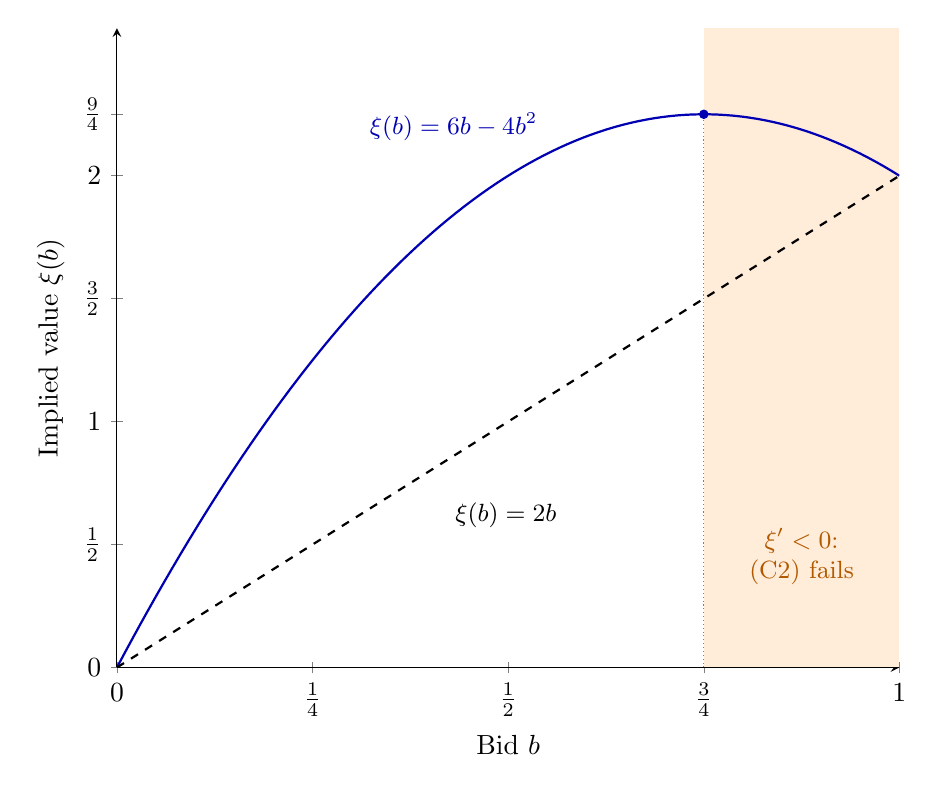
\begin{tikzpicture}
\begin{axis}[width=0.95\textwidth,height=0.8\textwidth,xmin=0,xmax=1,ymin=0,ymax=2.6,
  xlabel={Bid $b$},ylabel={Implied value $\xi(b)$},axis lines=left,
  xtick={0,0.25,0.5,0.75,1},xticklabels={$0$,$\frac14$,$\frac12$,$\frac34$,$1$},
  ytick={0,0.5,1,1.5,2,2.25},yticklabels={$0$,$\frac12$,$1$,$\frac32$,$2$,$\frac94$}]
\fill[orange!15] (axis cs:0.75,0) rectangle (axis cs:1,2.6);
\addplot[thick,blue!70!black,domain=0:1,samples=100] {6*x-4*x^2};
\addplot[thick,black,dashed,domain=0:1] {2*x};
\addplot[only marks,mark=*,mark size=1.5pt,blue!70!black] coordinates {(0.75,2.25)};
\draw[densely dotted,gray] (axis cs:0.75,0) -- (axis cs:0.75,2.25);
\node[font=\small,blue!70!black,anchor=east] at (axis cs:0.55,2.2) {$\xi(b)=6b-4b^2$};
\node[font=\small,anchor=west] at (axis cs:0.42,0.62) {$\xi(b)=2b$};
\node[font=\small,align=center,orange!70!black] at (axis cs:0.875,0.45) {$\xi'<0$:\\(C2) fails};
\end{axis}
\end{tikzpicture}
\caption{Inverse bid functions}
\end{subfigure}
\caption{The counterexample of \citet[p.~530]{GuerrePerrigneVuong2000}. Two bidders, bids i.i.d.\ with $G(b)=(\frac{b}{5-4b})^{\frac15}$ on $[0,1]$ (solid), against bids uniform on $[0,1]$ (dashed). The U-shaped bid density in panel (a) implies an inverse bid function that falls for $b>\frac34$ (shaded region in panel (b)), so no value distribution rationalizes these bids. Uniform bids imply $\xi(b)=2b$ and values uniform on $[0,2]$.}\label{fig:15-gpv-counter}
\end{figure}

\begin{remark}[What kind of identification result this is]\label{rem:15-gpv-ident-kind}
Four features of \cref{thm:15-gpv-ident} deserve emphasis. First, identification is nonparametric: no family of distributions is assumed. It implies identification within any parametric family. A parametric specification then serves only as an approximation and plays no role in identification (\cref{sec:15-identification}). Second, the proof is constructive, since \eqref{eq:15-gpv-F} gives $F$ explicitly. Third, the result is global. It does not rest on conditions in a neighborhood of a particular distribution \citep[footnote 7]{GuerrePerrigneVuong2000}. Fourth, the theorem characterizes the testable content of the model: (C1) and (C2) are all the restrictions that the SIPV first-price model places on bids from auctions with a fixed $n$. \Cref{sec:15-gpv-tests} turns them into tests.
\end{remark}

\begin{remark}[One equilibrium in all auctions]\label{rem:15-gpv-same-eq}
The inversion uses the distribution of rival bids observed across auctions as the belief of each bidder in each auction. This relies on the sampling assumption of \cref{sec:15-primitives} that the same equilibrium is played in all auctions with the same observables. In the SIPV model the equilibrium is unique, so the assumption holds automatically \citep[Section 3.1]{AtheyHaile2007}.
\end{remark}

\subsection{The bid density is smoother than the value density}\label{sec:15-gpv-smooth}

The estimator of \cref{sec:15-gpv-estimator} replaces $G$ and $g$ in \eqref{eq:15-gpv-xi} by estimates. How well they can be estimated depends on their smoothness. GPV show that the bid density has one more derivative than the value density.

\begin{proposition}[\citealp{GuerrePerrigneVuong2000}, Proposition 1]\label{prop:15-gpv-smooth}
Under \cref{ass:15-gpv-regularity}, the conditional bid distribution $G(\cdot\mid\cdot,\cdot)$ satisfies the following.
(i) For each $n\in\mathcal I$, its support is $\{(b,z):z\in[\underline z,\bar z],\ b\in[\underline b(z,n),\bar b(z,n)]\}$ with $\inf_z[\bar b(z,n)-\underline b(z,n)]>0$. The boundaries $\underline b(\cdot,n)$ and $\bar b(\cdot,n)$ have $R+1$ continuous bounded derivatives, and $\underline b(z,n)=\underline v(z)$.
(ii) $g(b\mid z,n)\ge c_g>0$ on the support.
(iii) $G(\cdot\mid\cdot,n)$ has $R+1$ continuous bounded partial derivatives on the support.
(iv) On any closed subset of the interior of the support, $g(\cdot\mid\cdot,n)$ has $R+1$ continuous bounded partial derivatives.
\end{proposition}

Part (iv) is the striking one. The value density has $R$ derivatives, and the bid density has $R+1$ on inner sets. The intuition comes from rearranging \eqref{eq:15-gpv-xi}:
\begin{equation}\label{eq:15-gpv-g-from-xi}
g(b\mid z,n)=\frac{G(b\mid z,n)}{(n-1)\big(\xi(b;z,n)-b\big)}
\end{equation}
\citep[p.~536]{GuerrePerrigneVuong2000}. The same formula appeared in \cref{sec:15-ml} as the bid density of a parametric model. The bid function \eqref{eq:15-gpv-rs} involves $F$ and its integral, so it has the $R+1$ derivatives of $F$. Its inverse $\xi$ inherits them. The distribution $G$ also has $R+1$ derivatives by part (iii). On inner sets the denominator of \eqref{eq:15-gpv-g-from-xi} is bounded away from zero, so $g$ has $R+1$ derivatives there. The bidding strategy acts as a smoothing operator. Each bid aggregates information about the whole lower tail of $F$ through the integral in \eqref{eq:15-gpv-rs}.

Formula \eqref{eq:15-gpv-g-from-xi} also explains part (ii) and the behavior of $g$ at the edges of its support. At the top, $G(\bar b)=1$, so $g(\bar b)=\frac{1}{(n-1)(\bar v-\bar b)}$. At the bottom, both $G$ and $\xi(b)-b$ vanish. To find the limit we expand near $\underline v$. Because $f(\underline v)>0$, we have $F(u)=f(\underline v)(u-\underline v)(1+o(1))$ as $u\downarrow\underline v$. Substituting into \eqref{eq:15-gpv-rs},
\[
v-\beta(v)=\frac{\int_{\underline v}^vf(\underline v)^{n-1}(u-\underline v)^{n-1}du}{f(\underline v)^{n-1}(v-\underline v)^{n-1}}\big(1+o(1)\big)=\frac{v-\underline v}{n}\big(1+o(1)\big).
\]
Hence, at $b=\beta(v)$,
\[
g(b)=\frac{F(v)}{(n-1)\big(v-\beta(v)\big)}=\frac{f(\underline v)(v-\underline v)}{(n-1)\frac{v-\underline v}{n}}\big(1+o(1)\big)\longrightarrow\frac{n}{n-1}\,f(\underline v)
\]
as $v\downarrow\underline v$. For values uniform on $[0,1]$, bids are uniform on $[0,\frac{n-1}{n}]$ with density $\frac{n}{n-1}$, which matches the formula.

The consequence for estimation is immediate. By \citet{Stone1982}, a function with $R+1$ derivatives in $d+1$ dimensions can be estimated uniformly at the rate $(\frac{T}{\log T})^{\frac{R+1}{2R+d+3}}$. The bid density, and with it the inverse bid function on inner sets, can therefore be estimated faster than the value density could be estimated even if values were observed. The difficulty lies elsewhere, as \cref{sec:15-gpv-rates} shows.

\subsection{The two-step estimator}\label{sec:15-gpv-estimator}

\Cref{thm:15-gpv-ident} suggests an estimator that mirrors identification. In the first step we estimate $G$ and $g$ nonparametrically and use \eqref{eq:15-gpv-xi} to build a \emph{pseudo-sample} of values, one pseudo-value per bid (\cref{sec:15-routes}). In the second step we treat the pseudo-values as a sample from $F$ and estimate its density by kernel smoothing. Kernel density estimation, bandwidths and boundary effects are reviewed in \cref{app:econometrics}. Throughout, kernels are normalized to have support $[-1,1]$.

\casehead{Homogeneous auctions} Suppose first that all $T$ auctions sell identical objects with the same number $n$ of bidders. The first step estimates the bid distribution by its empirical counterpart and the bid density by a kernel estimator (GPV, eqs.~(4)--(5)):
\begin{align}
\hat G(b)&=\frac{1}{nT}\sum_{t=1}^T\sum_{i=1}^n\indic(B_{it}\le b),\label{eq:15-gpv-Ghat}\\
\hat g(b)&=\frac{1}{nTh_g}\sum_{t=1}^T\sum_{i=1}^n\mathcal K\Big(\frac{b-B_{it}}{h_g}\Big),\label{eq:15-gpv-ghat}
\end{align}
where $\mathcal K$ is a kernel and $h_g$ a bandwidth. All $nT$ bids enter, because bids are i.i.d.\ within and across auctions under (C1).

\casehead{Boundary bias} A kernel density estimator is biased near the edges of the support, and the bias contaminates the pseudo-values. We derive the bias at the top of the support, following GPV, p.~531. Take a symmetric kernel with support $[-1,1]$ and a bid $b=\bar b-\lambda h_g$ with $\lambda\in[0,1)$. Then
\[
\E\big[\hat g(b)\big]=\frac{1}{h_g}\int_{\underline b}^{\bar b}\mathcal K\Big(\frac{b-y}{h_g}\Big)g(y)\,dy.
\]
We change variables to $u=\frac{b-y}{h_g}$, so that $y=b-h_gu$ and $dy=-h_g\,du$. The upper limit $y=\bar b$ becomes $u=\frac{b-\bar b}{h_g}=-\lambda$. The lower limit $y=\underline b$ becomes $u=\frac{b-\underline b}{h_g}$, which exceeds one once $h_g$ is small. Hence
\[
\E\big[\hat g(b)\big]=\int_{-\lambda}^{1}\mathcal K(u)\,g(b-h_gu)\,du\longrightarrow g(\bar b)\int_{-\lambda}^{1}\mathcal K(u)\,du\qquad\text{as }h_g\to0.
\]
For $\lambda<1$ the integral of the kernel is less than one, and at $\lambda=0$ it equals $\frac12$. Within one bandwidth of $\bar b$, the estimator therefore underestimates the density, by up to one half at the edge. The same argument applies within one bandwidth of $\underline b$.

The effect on the pseudo-values is large. At the top, $\hat G\approx1$ while $\hat g\approx\frac12g(\bar b)$, so the estimated markdown is about twice the true markdown $\bar v-\bar b$. The pseudo-value of the top bid is then about $\bar b+2(\bar v-\bar b)=2\bar v-\bar b$, well above the largest possible value. \Cref{fig:15-gpv-trim} shows the effect in a simulated sample.

\casehead{Trimming} Let $B_{\min}$ and $B_{\max}$ be the smallest and largest of the $nT$ bids. Because $\underline b\le B_{\min}$ and $B_{\max}\le\bar b$, the estimator $\hat g$ is asymptotically unbiased on $[B_{\min}+h_g,B_{\max}-h_g]$. GPV define the pseudo-values as (GPV, eq.~(6))
\begin{equation}\label{eq:15-gpv-trim}
\hat V_{it}=\begin{cases}
B_{it}+\dfrac{1}{n-1}\,\dfrac{\hat G(B_{it})}{\hat g(B_{it})}&\text{if }B_{\min}+h_g\le B_{it}\le B_{\max}-h_g,\\[2ex]
+\infty&\text{otherwise.}
\end{cases}
\end{equation}
Setting a trimmed pseudo-value to $+\infty$ removes it from the second step, because a kernel with bounded support assigns it zero weight.

\casehead{Second step} The density of values is estimated by (GPV, eq.~(7))
\begin{equation}\label{eq:15-gpv-fhat}
\hat f(v)=\frac{1}{nTh_f}\sum_{t=1}^T\sum_{i=1}^n\mathcal K_f\Big(\frac{v-\hat V_{it}}{h_f}\Big),
\end{equation}
with kernel $\mathcal K_f$ and bandwidth $h_f$. The distribution function, quantiles, and any functional of $F$ follow from the pseudo-values or from $\hat f$. The estimator involves no optimization and no equilibrium computation.

\casehead{Heterogeneous auctions} In applications the objects differ and the number of bidders varies. GPV, Section 3.3, extend the estimator jointly over $(b,z,n)$. Define
\[
G(b,z,n)=G(b\mid z,n)f_{Zn}(z,n),\qquad g(b,z,n)=g(b\mid z,n)f_{Zn}(z,n).
\]
The density $f_{Zn}$ cancels in the ratio, so \eqref{eq:15-gpv-xi} becomes (GPV, eq.~(12))
\begin{equation}\label{eq:15-gpv-psi}
V_{it}=B_{it}+\frac{1}{n_t-1}\,\psi(B_{it},Z_t,n_t),\qquad\psi(b,z,n)\equiv\frac{G(b,z,n)}{g(b,z,n)}.
\end{equation}
The ratio $\psi$ is a local symbol of this subsection, unrelated to the virtual valuation $\psi$ of \eqref{eq:14-psi}. The numerator and denominator are estimated by (GPV, eqs.~(13)--(14))
\begin{align}
\hat G(b,z,n)&=\frac{1}{Th_G^d}\sum_{t=1}^T\frac{1}{n_t}\sum_{i=1}^{n_t}\indic(B_{it}\le b)\,\mathcal K_G\Big(\frac{z-Z_t}{h_G},\frac{n-n_t}{h_{Gn}}\Big),\label{eq:15-gpv-Ghat-z}\\
\hat g(b,z,n)&=\frac{1}{Th_g^{d+1}}\sum_{t=1}^T\frac{1}{n_t}\sum_{i=1}^{n_t}\mathcal K_g\Big(\frac{b-B_{it}}{h_g},\frac{z-Z_t}{h_g},\frac{n-n_t}{h_{gn}}\Big).\label{eq:15-gpv-ghat-z}
\end{align}
The factor $\frac{1}{n_t}$ averages the bids within an auction, because $\E\big[\frac{1}{n_t}\sum_i\indic(B_{it}\le b)\mid Z_t,n_t\big]=G(b\mid Z_t,n_t)$. The kernels are products of kernels in each argument. The discrete variable $n$ receives its own bandwidths $h_{Gn}$ and $h_{gn}$, which vanish as $T$ grows, so that asymptotically only auctions with $n_t=n$ contribute \citep{Bierens1987}. With discrete covariates one estimates cell by cell, and $d$ counts only the continuous covariates \citep[footnote 12]{GuerrePerrigneVuong2000}.

\casehead{Estimated boundaries and trimming} The support of bids now varies with $(z,n)$ and is unknown. Even if $\underline v(\cdot)$ and $\bar v(\cdot)$ were known, $\bar b(z,n)=\beta(\bar v(z);z,n)$ would depend on $F$. GPV partition $\R^d$ into hypercubes of side $h_\partial$ and estimate (GPV, eqs.~(16)--(17))
\begin{align*}
\hat{\bar b}(z,n)&=\max\{B_{it}:\ Z_t\text{ in the hypercube containing }z,\ n_t=n\},\\
\hat{\underline b}(z)&=\min\{B_{it}:\ Z_t\text{ in the hypercube containing }z\}.
\end{align*}
The lower estimate pools all $n$, because $\underline b(z,n)=\underline v(z)$ does not depend on $n$. Let $\hat S_n=\{(b,z):z\in[\underline z,\bar z],\ b\in[\hat{\underline b}(z),\hat{\bar b}(z,n)]\}$ be the estimated support, and let $S(h)=[-h,h]^{d+1}$ denote the support of a kernel on $[-1,1]^{d+1}$ rescaled by $h$, a hypercube of side $2h$ centered at the origin. The kernel $\mathcal K_G$ does not smooth over bids, so for it GPV set the bid coordinate to zero, $S(h_G)=\{0\}\times[-h_G,h_G]^d$. The pseudo-value is $\hat V_{it}=B_{it}+\frac{1}{n_t-1}\hat\psi(B_{it},Z_t,n_t)$ with (GPV, eqs.~(18)--(19))
\begin{equation}\label{eq:15-gpv-trim-z}
\hat\psi(b,z,n)=\begin{cases}
\dfrac{\hat G(b,z,n)}{\hat g(b,z,n)}&\text{if }(b,z)+S(2h_G)\subset\hat S_n\text{ and }(b,z)+S(2h_g)\subset\hat S_n,\\[2ex]
+\infty&\text{otherwise.}
\end{cases}
\end{equation}
An observation is trimmed when the cube of half-width $2h_g$ centered at it leaves the estimated support, or when the corresponding cube of half-width $2h_G$ in the covariates does. Without covariates, the factor 2 can be replaced by 1. The condition $b+S(h_g)\subset[B_{\min},B_{\max}]$ then reads $B_{\min}+h_g\le b\le B_{\max}-h_g$, which returns \eqref{eq:15-gpv-trim} \citep[footnote 20]{GuerrePerrigneVuong2000}.

\casehead{Second step with covariates} The conditional density of values is the ratio $\hat f(v\mid z)=\frac{\hat f(v,z)}{\hat f(z)}$, where (GPV, eqs.~(20)--(21))
\begin{align}
\hat f(v,z)&=\frac{1}{Th_f^{d+1}}\sum_{t=1}^T\frac{1}{n_t}\sum_{i=1}^{n_t}\mathcal K_f\Big(\frac{v-\hat V_{it}}{h_f},\frac{z-Z_t}{h_f}\Big),\label{eq:15-gpv-fhat-z}\\
\hat f(z)&=\frac{1}{Th_Z^d}\sum_{t=1}^T\mathcal K_Z\Big(\frac{z-Z_t}{h_Z}\Big).\notag
\end{align}
The second step pools auctions with different $n$. This presumes that values and the number of bidders are independent given $Z_t$, so that $f(v\mid z,n)=f(v\mid z)$. GPV adopt this restriction and note that its failure calls for an explicit model of entry \citep[footnote 14]{GuerrePerrigneVuong2000}. \Cref{sec:15-entry} develops such models.

\begin{assumption}[Kernels and bandwidths, GPV Assumptions A3--A4]\label{ass:15-gpv-bandwidth}
(i) The kernels $\mathcal K_G$, $\mathcal K_g$, $\mathcal K_f$ and $\mathcal K_Z$ are symmetric with bounded hypercube supports, integrate to one, and have two continuous bounded derivatives in their continuous arguments. Their orders are $R+1$, $R+1$, $R$ and $R+1$, so that their moments of lower order vanish.
(ii) The discrete bandwidths $h_{Gn}$ and $h_{gn}$ vanish as $T\to\infty$.
(iii) For positive constants $c_G,c_g,c_f,c_Z,c_\partial$,
\begin{align*}
h_G&=c_G\Big(\frac{\log T}{T}\Big)^{\frac{1}{2R+d+2}}, & h_g&=c_g\Big(\frac{\log T}{T}\Big)^{\frac{1}{2R+d+3}},\\
h_f&=c_f\Big(\frac{\log T}{T}\Big)^{\frac{1}{2R+d+3}}, & h_Z&=c_Z\Big(\frac{\log T}{T}\Big)^{\frac{1}{2R+d+2}},
\end{align*}
and, when $d>0$, $h_\partial=c_\partial\big(\frac{\log T}{T}\big)^{\frac{1}{d+1}}$.
\end{assumption}

The bandwidths for $G$, $g$ and $f(z)$ are the uniformly optimal choices for functions with $R+1$ derivatives. A function of $d$ arguments with $R+1$ derivatives calls for the exponent $\frac{1}{2(R+1)+d}=\frac{1}{2R+d+2}$. The bid density has $d+1$ arguments, which gives $\frac{1}{2R+d+3}$. The factor $\log T$ appears because the results concern uniform convergence. The choice of $h_f$ is unusual. If values were observed, the optimal exponent for $f(\cdot,\cdot)$ would be $\frac{1}{2R+d+1}$, and $h_f$ would shrink faster. The prescribed $h_f$ is larger, so the second step \emph{oversmooths}. \Cref{sec:15-gpv-rates} explains why this is the only rate that attains the optimal convergence rate.

\casehead{Bandwidths in practice} GPV's Monte Carlo uses $R=1$ and $d=0$, so both $h_g$ and $h_f$ are of order $T^{-\frac15}$ up to the logarithm. They use the triweight kernel
\[
\mathcal K(u)=\frac{35}{32}\big(1-u^2\big)^3\indic(|u|\le1)
\]
for both steps, with $h_g=1.06\,\hat\sigma_b(nT)^{-\frac15}$ and $h_f=1.06\,\hat\sigma_v(nT_T)^{-\frac15}$ \citep[p.~532]{GuerrePerrigneVuong2000}. Here $\hat\sigma_b$ and $\hat\sigma_v$ are the standard deviations of the bids and of the pseudo-values that survive trimming, which GPV call the trimmed pseudo private values. $T_T$ is the number of auctions left after trimming. The factor 1.06 is the Gaussian rule of thumb \citep{Hardle1991}.

Later work multiplies the rule by $2.978$ when it uses the triweight kernel \citep{LiPerrigneVuong2002,CampoPerrigneVuong2003,Krasnokutskaya2011}. The factor converts a bandwidth that is optimal for the Gaussian kernel into the equivalent bandwidth for the triweight kernel. We verify it. For a second-order kernel, the bandwidth that minimizes the asymptotic mean integrated squared error is proportional to the kernel constant $\delta_{\mathcal K}=\big(\frac{\int\mathcal K^2}{(\int u^2\mathcal K)^2}\big)^{\frac15}$. The factor of proportionality does not depend on the kernel \citep{Hardle1991}. For the Gaussian kernel, $\int\mathcal K^2=\frac{1}{2\sqrt\pi}$ and $\int u^2\mathcal K=1$, so $\delta=(2\sqrt\pi)^{-\frac15}\approx0.7764$. For the triweight kernel,
\[
\int_{-1}^1\mathcal K^2=\Big(\frac{35}{32}\Big)^2\int_{-1}^1(1-u^2)^6du=\frac{350}{429},\qquad\int_{-1}^1u^2\mathcal K=\frac{35}{32}\int_{-1}^1u^2(1-u^2)^3du=\frac19,
\]
so $\delta=\big(\frac{350}{429}\cdot81\big)^{\frac15}\approx2.3122$. The ratio is $\frac{2.3122}{0.7764}\approx2.978$. GPV's choice, without the factor, is narrower than the Gaussian-equivalent bandwidth. It trims fewer bids and smooths less. \Cref{tab:15-gpv-mc} compares the two choices.

\casehead{The algorithm} For a sample of first-price auctions with all bids recorded, the estimator proceeds as follows.
\begin{enumerate}
\item Group auctions by the number of bidders, and by covariate cells if covariates are discrete. Choose kernels and bandwidths, for example by the rule of thumb above.
\item For each bid, compute $\hat G(B_{it})$ and $\hat g(B_{it})$ from \eqref{eq:15-gpv-Ghat}--\eqref{eq:15-gpv-ghat}, or from \eqref{eq:15-gpv-Ghat-z}--\eqref{eq:15-gpv-ghat-z} with continuous covariates.
\item Trim the bids within one bandwidth of the estimated boundaries, and compute the pseudo-values of the remaining bids from \eqref{eq:15-gpv-trim} or \eqref{eq:15-gpv-trim-z}.
\item Evaluate $\hat\xi(b)=b+\frac{\hat G(b)}{(n-1)\hat g(b)}$ on a grid and check that it is increasing, as (C2) requires.
\item Estimate the value density by \eqref{eq:15-gpv-fhat} or \eqref{eq:15-gpv-fhat-z}, and compute the functionals of interest. Examples are value quantiles, the winner's informational rent $\frac{V-B}{V}$, the optimal reserve price from $\hat F$ (\cref{cor:14-optimal-reserve}), and expected revenue under other formats, such as $\E[V^{(n-1:n)}]$ for a second-price auction.
\end{enumerate}

\subsection{Rates of convergence and inference*}\label{sec:15-gpv-rates}

How fast can any estimator recover $f(\cdot\mid z)$ from bids? GPV answer with the minimax theory of \citet{IbragimovHasminskii1981}. We state the criterion, the result, and a sketch of the proof. Let $\mathcal C$ be a compact subset, with nonempty interior, of the interior of the support of $f_0(v,z)$. For a candidate rate $r_T\to\infty$, consider (GPV, eq.~(10))
\begin{equation}\label{eq:15-gpv-minimax}
\inf_{\hat f}\ \sup_{f\in U_\epsilon(f_0)}\Pr_f\Big(r_T\sup_{(v,z)\in\mathcal C}\big|\hat f(v\mid z)-f(v\mid z)\big|>\kappa\Big),
\end{equation}
where the infimum runs over all estimators based on bids. Here $\Pr_f$ is the law of the observables when values have density $f$. The neighborhood $U_\epsilon(f_0)$ contains the densities that satisfy \cref{ass:15-gpv-regularity}, lie within $\epsilon$ of $f_0$ in sup norm, and have derivatives up to order $R$ bounded by a constant $M$. Taking the supremum over a neighborhood rules out estimators that do well at one density only. If $r_T$ grows too fast, \eqref{eq:15-gpv-minimax} stays bounded away from zero for every estimator. The optimal uniform rate is the fastest $r_T$ for which some estimator drives \eqref{eq:15-gpv-minimax} to zero for large $\kappa$.

\begin{theorem}[\citealp{GuerrePerrigneVuong2000}, Theorems 2 and 3]\label{thm:15-gpv-rate}
Let \cref{ass:15-gpv-sampling} and \cref{ass:15-gpv-regularity} hold.
\begin{itemize}
\item[(i)] (Lower bound.) There is $\kappa>0$ such that, with $r_T=(\frac{T}{\log T})^{\frac{R}{2R+d+3}}$,
\[
\lim_{\epsilon\to0}\ \liminf_{T\to\infty}\ \inf_{\hat f}\ \sup_{f\in U_\epsilon(f_0)}\Pr_f\Big(r_T\sup_{(v,z)\in\mathcal C}\big|\hat f(v\mid z)-f(v\mid z)\big|>\kappa\Big)>0.
\]
\item[(ii)] (Attainment.) If, in addition, \cref{ass:15-gpv-bandwidth} holds, the two-step estimator satisfies, for every closed inner subset $\mathcal C$ of the support,
\[
\sup_{(v,z)\in\mathcal C}\big|\hat f(v\mid z)-f(v\mid z)\big|=O\Big(\Big(\frac{\log T}{T}\Big)^{\frac{R}{2R+d+3}}\Big)\quad\text{almost surely}.
\]
\end{itemize}
Hence $(\frac{T}{\log T})^{\frac{R}{2R+d+3}}$ is the optimal uniform rate for estimating $f(\cdot\mid\cdot)$ from bids, and the two-step estimator attains it.
\end{theorem}

If values were observed, the optimal uniform rate would be $(\frac{T}{\log T})^{\frac{R}{2R+d+1}}$ \citep{Stone1982}. Not observing values costs two units in the denominator of the exponent. The proof of part (i) adapts the argument of \citet{Khasminskii1976} and relies on \cref{thm:15-gpv-ident,prop:15-gpv-smooth}. We do not reproduce it.

\casehead{Where the loss comes from} Differentiating \eqref{eq:15-gpv-F} with respect to $v$ gives (GPV, eq.~(11))
\begin{equation}\label{eq:15-gpv-f-from-xi}
f(v\mid z,n)=\frac{g\big(\xi^{-1}(v;z,n)\mid z,n\big)}{\xi'\big(\xi^{-1}(v;z,n);z,n\big)}.
\end{equation}
Recovering $f$ requires the derivative $\xi'$, and by \eqref{eq:15-gpv-xi} this requires the derivative $g'$. The bid density has $R+1$ derivatives in $d+1$ arguments. By \citet{Stone1982}, the optimal uniform rate for the first derivative of such a function is $(\frac{T}{\log T})^{\frac{(R+1)-1}{2(R+1)+(d+1)}}=(\frac{T}{\log T})^{\frac{R}{2R+d+3}}$. Estimating $g'$ is the hardest part of the problem, and its rate is the rate for $f$. \Cref{tab:15-gpv-rates} compares the exponents.

\begin{table}[htbp]
\centering
\begin{threeparttable}
\caption{Exponents of the optimal uniform convergence rates $(\frac{T}{\log T})^{a}$}\label{tab:15-gpv-rates}
\small
\begin{tabular}{ccccc}
\toprule
$R$ & $d$ & \makecell{Values observed\\ $a=\frac{R}{2R+d+1}$} & \makecell{Bids only\\ $a=\frac{R}{2R+d+3}$} & \makecell{Pseudo-values, inner sets\\ $a=\frac{R+1}{2R+d+3}$}\\
\midrule
1 & 0 & $\frac13$ & $\frac15$ & $\frac25$\\[2pt]
2 & 0 & $\frac25$ & $\frac27$ & $\frac37$\\[2pt]
1 & 1 & $\frac14$ & $\frac16$ & $\frac13$\\[2pt]
2 & 1 & $\frac13$ & $\frac14$ & $\frac38$\\[2pt]
1 & 2 & $\frac15$ & $\frac17$ & $\frac27$\\
\bottomrule
\end{tabular}
\begin{tablenotes}
\footnotesize
\item \textit{Notes.} $R$ is the number of bounded derivatives of the value density and $d$ the number of continuous covariates. The column ``Values observed'' gives the rate of \citet{Stone1982}, and the column ``Bids only'' gives the rate of \cref{thm:15-gpv-rate}. The last column gives the rate of $\sup|\hat V_{it}-V_{it}|$ over bids away from the boundary (GPV, Proposition 3(ii)). Our computation from these formulas.
\end{tablenotes}
\end{threeparttable}
\end{table}

\casehead{Sketch of the proof of part (ii)} The argument shows why the second step must oversmooth. Write $\varepsilon_T=\frac{\log T}{T}$. Two preliminary results are needed. The boundary estimators converge at the rate $\varepsilon_T^{\frac{1}{d+1}}$ (GPV, Proposition 2). The untrimmed pseudo-values satisfy $\sup|\hat V_{it}-V_{it}|=O(\varepsilon_T^{\frac{R}{2R+d+3}})$, and on bids away from the boundary $\sup|\hat V_{it}-V_{it}|=O(\varepsilon_T^{\frac{R+1}{2R+d+3}})$ almost surely (GPV, Proposition 3). The faster inner rate reflects the extra derivative of $g$ in \cref{prop:15-gpv-smooth}.

Because $\hat f(z)$ converges at the faster rate $\varepsilon_T^{\frac{R+1}{2R+d+2}}$ and $f(z)$ is bounded away from zero, it suffices to study $\hat f(v,z)$. Let $\tilde f(v,z)$ be the infeasible estimator \eqref{eq:15-gpv-fhat-z} computed with the true values $V_{it}$ in place of $\hat V_{it}$ (GPV, eq.~(22)). We decompose
\[
\hat f(v,z)-f(v,z)=\big[\hat f(v,z)-\tilde f(v,z)\big]+\big[\tilde f(v,z)-f(v,z)\big].
\]
The second bracket is the error of an ordinary kernel estimator. Its bias is $O(h_f^R)$, since $\mathcal K_f$ has order $R$ and $f$ has $R$ derivatives. Its stochastic part is $O\big((\frac{\log T}{Th_f^{d+1}})^{\frac12}\big)$ uniformly. With $h_f\propto\varepsilon_T^{\frac{1}{2R+d+3}}$, these are
\[
h_f^R\propto\varepsilon_T^{\frac{R}{2R+d+3}},\qquad\Big(\frac{\varepsilon_T}{h_f^{d+1}}\Big)^{\frac12}\propto\varepsilon_T^{\frac12\left(1-\frac{d+1}{2R+d+3}\right)}=\varepsilon_T^{\frac{R+1}{2R+d+3}}.
\]
The bias dominates, and the second bracket is $O(\varepsilon_T^{\frac{R}{2R+d+3}})$.

For the first bracket, points $(v,z)$ in $\mathcal C$ use only observations whose true values lie in a slightly larger inner set, once $T$ is large. A second-order Taylor expansion of $\mathcal K_f$ in its first argument gives (GPV, eq.~(23))
\[
\big|\hat f(v,z)-\tilde f(v,z)\big|\le\frac{\sup|\hat V_{it}-V_{it}|}{h_f}\,A_T+\frac{\sup|\hat V_{it}-V_{it}|^2}{2h_f^3}\,B_T,
\]
where the suprema run over inner observations. The terms $A_T$ and $B_T$ are averages of the type $\frac{1}{Th_f^{d+1}}\sum_t|\partial_1\mathcal K_f(\cdot)|$ and $\frac{1}{Th_f^{d}}\sum_t\sup_v|\partial_1^2\mathcal K_f(\cdot)|$. Like kernel estimators, they stay bounded almost surely. Using the inner rate of Proposition 3, the first term is of order
\[
\frac{\varepsilon_T^{\frac{R+1}{2R+d+3}}}{\varepsilon_T^{\frac{1}{2R+d+3}}}=\varepsilon_T^{\frac{R}{2R+d+3}},
\]
and the second is of order $\varepsilon_T^{\frac{2(R+1)-3}{2R+d+3}}=\varepsilon_T^{\frac{2R-1}{2R+d+3}}$. Since $R\ge1$ implies $2R-1\ge R$, the second term is no larger than the first. Both brackets are therefore $O(\varepsilon_T^{\frac{R}{2R+d+3}})$, which proves part (ii).

The bookkeeping explains the choice of $h_f$. The first-step error enters as $\frac{\sup|\hat V-V|}{h_f}$, which falls as $h_f$ grows. The smoothing bias $h_f^R$ rises with $h_f$. Equating $\varepsilon_T^{\frac{R+1}{2R+d+3}}h_f^{-1}$ with $h_f^R$ gives $h_f^{R+1}=\varepsilon_T^{\frac{R+1}{2R+d+3}}$, that is $h_f\propto\varepsilon_T^{\frac{1}{2R+d+3}}$. Given the optimal first-step bandwidths, this is the only rate for $h_f$ that attains the optimal rate \citep[p.~546]{GuerrePerrigneVuong2000}. The usual choice $h_f\propto\varepsilon_T^{\frac{1}{2R+d+1}}$ would undersmooth relative to the first-step noise and give a slower rate.

\casehead{Inference} \Cref{thm:15-gpv-rate} gives rates of convergence. It says nothing about limiting distributions, and GPV do not establish asymptotic normality of $\hat f$. They note that the second-order term of the expansion can be close to the first when $R$ is small, so normal approximations based on the leading term may be inaccurate \citep[p.~546]{GuerrePerrigneVuong2000}. They suggest instead an exponential inequality of the form (GPV, eq.~(24))
\[
\Pr\Big(\Big(\frac{T}{\log T}\Big)^{\frac{R}{2R+d+3}}\sup_{(v,z)\in\mathcal C}\big|\hat f(v\mid z)-f(v\mid z)\big|>e^*(\tau)\Big)\le P^*(\tau),
\]
which would deliver conservative uniform bands $\hat f\pm e^*(\tau)(\frac{\log T}{T})^{\frac{R}{2R+d+3}}$ with coverage at least $1-P^*(\tau)$. The same inequality bounds the expected sup-norm loss and could guide the choice of the bandwidth constants. GPV leave the derivation of $e^*$ and $P^*$ to future work.

Practice has moved in two directions \citep[Section 3.2.1]{AtheyHaile2007}. First, many questions concern functionals of $F$, such as quantiles, expected revenue or the optimal reserve price. \Citet{HaileHongShum2003} show that the pseudo-values and fixed quantiles of their empirical distribution are asymptotically normal. Second, applied work uses the bootstrap. Outside the IPV model, bids are correlated within an auction. One therefore resamples whole auctions with replacement within each value of $n$ and recomputes both steps in each bootstrap sample. Subsampling is an alternative \citep{HaileHongShum2003}.

\subsection{A Monte Carlo illustration*}\label{sec:15-gpv-mc}

\casehead{GPV's design} GPV illustrate the estimator with a small Monte Carlo study \citep[Section 2.4]{GuerrePerrigneVuong2000}. Each replication has $T=200$ auctions with $n=5$ bidders, so 1,000 bids, which they describe as a realistic sample size. Values are lognormal with parameters zero and one, truncated to $[0.055,2.5]$. GPV say that the truncation leaves out ``20\% approximately'' of the original lognormal distribution (p.~532). Our calculation gives 18.2 percent, almost all of it above 2.5. The truncation makes the support compact as \cref{ass:15-gpv-regularity} requires. Bids are computed from \eqref{eq:15-gpv-rs} by numerical integration. The estimator uses $R=1$, triweight kernels in both steps, and the rule-of-thumb bandwidths described in \cref{sec:15-gpv-estimator}. There are 1,000 replications.

GPV report the results in two figures, without tables. Their Figure~1 plots the true equilibrium strategy with the mean and the 5th and 95th percentiles of the 1,000 estimates $\hat\xi(b)$, evaluated at 500 points on $[\beta(0.055),\beta(2.5)]$. Their Figure~2 does the same for the density on $[0.055,2.5]$. Inside the region delimited by the trimming, the true curves lie within the pointwise 90 percent bands and the mean estimates match them closely \citep[p.~533]{GuerrePerrigneVuong2000}. Each replication took less than a minute in FORTRAN. GPV estimate that a parametric nonlinear least squares estimator would take about 1,000 times longer, because it requires the numerical integration of \eqref{eq:15-gpv-rs} at every trial parameter \citep[p.~532]{GuerrePerrigneVuong2000}.

\casehead{Our replication} We replicate the design exactly, including the bandwidth rules with the factor 1.06 and 1,000 replications. The script \texttt{figures/ch15/src/gpv\_montecarlo.py} computes the true bid function by integrating \eqref{eq:15-gpv-rs} on a grid of 200,001 points, with seed 15401. \Cref{fig:15-gpv-mc} reports the results in the format of GPV's Figures 1 and 2. As in their footnote~9, the dotted lines mark the average trimming bounds $B_{\min}+h_g$ and $B_{\max}-h_g$ in panel (a). In panel (b) they mark the average of $\hat\xi(B_{\min}+h_g)+h_f$ and $\hat\xi(B_{\max}-h_g)-h_f$, which removes the remaining boundary effects of the second step.

\begin{figure}[htbp]
\centering
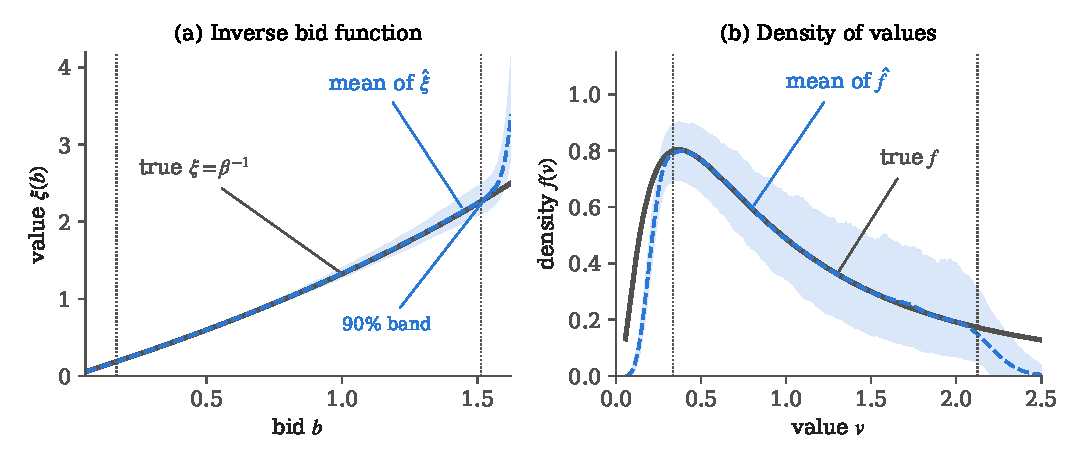
\includegraphics[width=\textwidth]{figures/ch15/gpv_mc.pdf}
\caption{Replication of the Monte Carlo design of \citet[Section 2.4]{GuerrePerrigneVuong2000}: $T=200$ auctions, $n=5$ bidders, values lognormal$(0,1)$ truncated to $[0.055,2.5]$, triweight kernels, $h_g=1.06\,\hat\sigma_b(nT)^{-\frac15}$, $h_f=1.06\,\hat\sigma_v(nT_T)^{-\frac15}$, 1,000 replications. Panel (a): true inverse bid function, mean of $\hat\xi(b)$ (dashed) and pointwise 90 percent band of the estimates. Panel (b): true value density, mean of $\hat f(v)$ and 90 percent band. Dotted lines mark the average trimming bounds. Our simulation (seed 15401), following the design of \citet[Section 2.4]{GuerrePerrigneVuong2000}.}\label{fig:15-gpv-mc}
\end{figure}

The replication reproduces GPV's qualitative findings. Inside the dotted lines the mean estimates are close to the truth, and the true curves lie inside the bands at every grid point. On the trimmed bid range, the mean of $\hat\xi$ is never more than 0.013 away from $\xi$. On the inner value region, the mean of $\hat f$ is never more than 0.022 away from $f$ (\cref{tab:15-gpv-mc}). The average trimming bounds on bids are 0.168 and 1.511, and the inner value region is $[0.334,2.125]$. Both are close to the lines drawn in GPV's figures. Outside these regions the estimates deteriorate as \cref{sec:15-gpv-estimator} predicts. Near the top of the bid support the mean of $\hat\xi$ bends sharply upward. Near both ends of the value support the mean of $\hat f$ falls below the truth.

\begin{figure}[htbp]
\centering
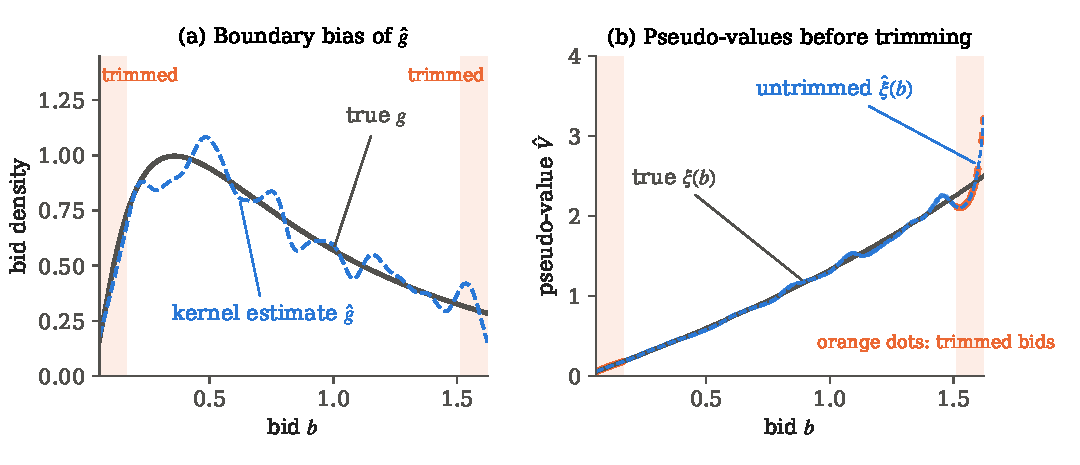
\includegraphics[width=\textwidth]{figures/ch15/gpv_trim.pdf}
\caption{Boundary effects in one simulated sample from the design of \cref{fig:15-gpv-mc} ($h_g=0.108$). Panel (a): true bid density and the triweight kernel estimate. Shaded areas lie within one bandwidth of the smallest and largest bids. At the largest bid the estimate equals 0.54 times the true density. Panel (b): pseudo-values $B_{it}+\frac{\hat G(B_{it})}{(n-1)\hat g(B_{it})}$ before trimming (dots), the estimated inverse bid function on a grid (dashed) and the true $\xi$ (solid). Near the top, the underestimated density inflates the markdown, and the estimated inverse bid function rises well above $\bar v=2.5$. Our simulation (seed 15403).}\label{fig:15-gpv-trim}
\end{figure}

\Cref{fig:15-gpv-trim} shows the mechanism in one sample. At the largest bid, $\hat g$ is 0.54 times the true density, close to the factor $\frac12$ derived in \cref{sec:15-gpv-estimator}. The untrimmed estimate $\hat\xi$ climbs to about 3.2 at the top of the bid support, against a true maximum value of 2.5. Trimming removes 43 of the 1,000 bids at the top. Among the bids that survive trimming, the mean absolute error of the pseudo-values is 0.016.

\begin{table}[htbp]
\centering
\caption{Monte Carlo results for the GPV estimator}\label{tab:15-gpv-mc}
\small
\begin{tabular}{lcc}
\toprule
\multicolumn{3}{l}{\textit{Panel A. GPV design, $T=200$, $n=5$, 1,000 replications}}\\
\midrule
Bandwidth constant & $1.06$ (GPV) & $2.978\times1.06$ \\
\midrule
Mean $h_g$ & 0.107 & 0.320\\
Mean $h_f$ & 0.147 & 0.334\\
Share of bids trimmed & 0.088 & 0.363\\
Mean trimming bounds on bids & $[0.168,\,1.511]$ & $[0.380,\,1.299]$\\
Inner value region & $[0.334,\,2.125]$ & $[0.781,\,1.508]$\\
Max.\ $|$mean of $\hat\xi-\xi|$ on trimmed bids & 0.013 & 0.003\\
Max.\ $|$mean of $\hat f-f|$ on inner values & 0.022 & 0.006\\
Mean sup-norm error of $\hat\xi$ on trimmed bids & 0.161 & 0.043\\
Mean sup-norm error of $\hat f$ on inner values & 0.238 & 0.055\\
Seconds per replication (Python) & 0.028 & 0.076\\
\bottomrule
\end{tabular}

\medskip
\begin{tabular}{rcccc}
\toprule
\multicolumn{5}{l}{\textit{Panel B. Mean sup-norm errors on fixed inner sets, GPV bandwidths, 200 replications}}\\
\midrule
$T$ & \makecell{$\hat\xi$, bids\\ in $[0.25,1.35]$} & \makecell{$\hat f$, values\\ in $[0.4,1.8]$} & \makecell{$\tilde f$\\ (true values)} & Ratio $\frac{\hat f}{\tilde f}$\\
\midrule
100 & 0.149 & 0.243 & 0.128 & 1.89\\
200 & 0.113 & 0.227 & 0.102 & 2.21\\
400 & 0.087 & 0.203 & 0.080 & 2.54\\
800 & 0.067 & 0.176 & 0.064 & 2.73\\
1,600 & 0.053 & 0.152 & 0.049 & 3.07\\
\midrule
Log-log slope in $T$ & $-0.37$ & $-0.17$ & $-0.34$ & \\
\bottomrule
\end{tabular}

\smallskip
\begin{minipage}{0.9\textwidth}
\footnotesize
\textit{Notes.} Our simulation, script \texttt{figures/ch15/src/gpv\_montecarlo.py}, seeds 15401 (panel A) and 15402 (panel B). Values lognormal$(0,1)$ truncated to $[0.055,2.5]$, $n=5$, triweight kernels. In panel A the two columns use the same draws. The inner value region is the average of $[\hat\xi(B_{\min}+h_g)+h_f,\ \hat\xi(B_{\max}-h_g)-h_f]$, so the error rows of the two columns refer to different regions. In panel B, $\tilde f$ is the infeasible kernel estimator computed from the true values with the same kernel and rule-of-thumb bandwidth. Slopes are least-squares fits of the log error on $\log T$. Timings are from one run on a laptop and vary across runs.
\end{minipage}
\end{table}

Panel A of \cref{tab:15-gpv-mc} compares GPV's bandwidths with the Gaussian-equivalent bandwidths. The wider bandwidths cut the sup-norm errors by a factor of about four. They do so at a price: 36 percent of the bids are trimmed, and the inner value region shrinks to $[0.781,1.508]$. The tails of $F$, which matter for reserve prices and for the top of the bid distribution, are then not estimated at all. The trade-off between precision in the middle and coverage of the support is a practical feature of every application of the method.

Panel B illustrates \cref{thm:15-gpv-rate}. On fixed inner sets, the error of $\hat f$ falls more slowly with $T$ than the error of the infeasible estimator that uses true values. The ratio of the two errors rises from 1.9 at $T=100$ to 3.1 at $T=1{,}600$. The fitted slope for $\hat f$ is $-0.17$, close to the exponent $-\frac15$ that the theorem gives for $R=1$ and $d=0$. The slope for $\tilde f$ is $-0.34$. The inverse bid function requires $g$ without its derivative, and its error falls at the faster slope of $-0.37$. The design has a very smooth density, so these slopes illustrate the theory. They are no test of it. The whole experiment takes a few minutes on a laptop, which makes the computational case for the indirect approach plain.

\subsection{Binding reserve prices and unknown numbers of potential bidders}\label{sec:15-gpv-reserve}

In practice sellers often announce a reserve price high enough to screen out some bidders. GPV, Section 4, extend their results to this case. A binding reserve price creates a new unknown. Let $N$ denote the number of \emph{potential bidders}, who draw values and decide whether to bid. Let $n^*$ denote the number of \emph{actual bidders}, who submit a bid of at least $r$. The econometrician observes $n^*$ but typically not $N$. Following GPV, bidders do not observe which rivals participate when they bid.

\casehead{The inverse bid function with a reserve} Fix one auction with reserve price $r\in(\underline v,\bar v)$. Bidders with values below $r$ do not bid, and bidders with values $v\ge r$ bid $\beta(v)$ from \eqref{eq:14-rs-bid}, with $\beta(r)=r$. Let $G^*$ denote the distribution of an actual bid, with density $g^*$ on $[r,\bar b]$. Then
\[
G^*(b)=\Pr\big(\beta(V)\le b\bigm| V\ge r\big)=\frac{F\big(\beta^{-1}(b)\big)-F(r)}{1-F(r)}.
\]
We derive the analog of \eqref{eq:15-gpv-xi} from the bidder's problem. A bid $b\ge r$ beats a given rival if that rival's value is below $r$, which has probability $F(r)$, or if the rival bids but bids less than $b$, which has probability $(1-F(r))G^*(b)$. Rivals are independent, so the win probability is
\[
H(b)=\Big[F(r)+\big(1-F(r)\big)G^*(b)\Big]^{N-1}.
\]
The bidder maximizes $(v-b)H(b)$. The first-order condition is
\[
(v-b)(N-1)\Big[F(r)+\big(1-F(r)\big)G^*(b)\Big]^{N-2}\big(1-F(r)\big)g^*(b)=\Big[F(r)+\big(1-F(r)\big)G^*(b)\Big]^{N-1}.
\]
Dividing by $(N-1)[F(r)+(1-F(r))G^*(b)]^{N-2}(1-F(r))g^*(b)$ and adding $b$ gives
\[
v=b+\frac{F(r)+\big(1-F(r)\big)G^*(b)}{(N-1)\big(1-F(r)\big)g^*(b)}.
\]
Splitting the fraction yields GPV's equation~(25):
\begin{equation}\label{eq:15-gpv-reserve}
v=\xi\big(b;G^*,N,F(r)\big)\equiv b+\frac{1}{N-1}\Big(\frac{G^*(b)}{g^*(b)}+\frac{F(r)}{1-F(r)}\,\frac{1}{g^*(b)}\Big).
\end{equation}
The second term in the parentheses reflects the potential bidders who do not bid. Ignoring it understates the markdown, especially near $r$, where $G^*$ is small. Unlike \eqref{eq:15-gpv-xi}, equation \eqref{eq:15-gpv-reserve} involves two unknowns, $N$ and $F(r)$.

\casehead{Why the bid density is unbounded at the reserve} By \eqref{eq:15-gpv-ode} with $N$ bidders, $\beta'(v)=(N-1)\frac{f(v)}{F(v)}\big(v-\beta(v)\big)$. At $v=r$ the markdown $v-\beta(v)$ vanishes while $F(r)>0$, so $\beta'(r)=0$. Let $\Delta(v)=v-\beta(v)$. Then $\Delta(r)=0$ and $\Delta'(r)=1-\beta'(r)=1$, so $\Delta(v)=(v-r)(1+o(1))$. Substituting,
\[
\beta'(v)=(N-1)\frac{f(r)}{F(r)}(v-r)\big(1+o(1)\big),\qquad\beta(v)-r=\frac{(N-1)f(r)}{2F(r)}(v-r)^2\big(1+o(1)\big).
\]
The bid function is flat and quadratic near the reserve. Many values just above $r$ map into a short interval of bids, and the density $g^*(b)=\frac{f(v)}{\beta'(v)(1-F(r))}$ behaves like $(b-r)^{-\frac12}$ as $b\downarrow r$ \citep[p.~549]{GuerrePerrigneVuong2000}.

\begin{theorem}[\citealp{GuerrePerrigneVuong2000}, Theorem 4]\label{thm:15-gpv-reserve}
Let $G^*\in\mathcal P$ have support $[r,\bar b]$, and let $\mathcal Q$ be a discrete distribution on $\{0,1,2,\dots\}$. Consider a first-price SIPV auction with reserve price $r\in(\underline v,\bar v)$. There exist $F\in\mathcal P$ and $N\ge2$ that generate $G^*$ as the distribution of actual bids and $\mathcal Q$ as the distribution of the number of actual bidders if and only if the following hold.
\begin{itemize}
\item[(C1)] $\mathcal Q$ is binomial with parameters $(N,1-F(r))$, where $0<F(r)<1$.
\item[(C2)] Conditional on $n^*$, actual bids are i.i.d.\ with distribution $G^*$, and $g^*(b)\to+\infty$ as $b\downarrow r$.
\item[(C3)] The function $\xi(\cdot;G^*,N,F(r))$ in \eqref{eq:15-gpv-reserve} is strictly increasing on $[r,\bar b]$, and its inverse is differentiable on $[r,\bar v]\equiv[\xi(r),\xi(\bar b)]$.
\end{itemize}
If (C1)--(C3) hold, $N$ and $F(r)$ are unique, and $F$ is unique on $[r,\bar v]$, with
\[
F(v)=F(r)+\big(1-F(r)\big)G^*\big(\xi^{-1}(v;G^*,N,F(r))\big).
\]
Moreover, $\xi(\cdot;G^*,N,F(r))$ is the inverse of the equilibrium strategy on $[r,\bar b]$.
\end{theorem}

\begin{proof}[Sketch of proof]
Necessity of (C1) holds because each potential bidder bids independently with probability $1-F(r)$. For (C2), consider $k$ actual bidders. Exchangeability and independence give
\[
\Pr\big(B^*_1\le b_1,\dots,B^*_k\le b_k\bigm| n^*=k\big)=\frac{\binom Nk F(r)^{N-k}\prod_{j=1}^k\Pr(r\le B_j\le b_j)}{\binom Nk F(r)^{N-k}\big(1-F(r)\big)^k}=\prod_{j=1}^k\frac{F\big(\beta^{-1}(b_j)\big)-F(r)}{1-F(r)}.
\]
The unbounded density follows from $\beta'(r)=0$, as shown above. Necessity of (C3) follows as in \cref{thm:15-gpv-ident}, because \eqref{eq:15-gpv-reserve} is the first-order condition. For sufficiency, (C1) identifies $N$ and $F(r)$, as in \cref{prop:15-reserve-ident}(iii): the mean and variance of $n^*$ are $N(1-F(r))$ and $NF(r)(1-F(r))$. The rest of the argument repeats the proof of \cref{thm:15-gpv-ident} with the truncated distributions $G^*$ and $\frac{F-F(r)}{1-F(r)}$. The condition $g^*\to\infty$ plays the role of \eqref{eq:15-gpv-A1}: it gives $\lim_{b\downarrow r}\xi(b)=r$, so that the candidate strategy satisfies $\beta(r)=r$. Below $r$, any absolutely continuous extension of $F$ rationalizes the data. GPV, Appendix A.1, give the details.
\end{proof}

The theorem parallels \cref{thm:15-gpv-ident}. The data identify the number of potential bidders and the probability of not bidding. The value distribution is identified only above the reserve price. Below $r$ the data contain no information about $F$ beyond the mass $F(r)$.

\casehead{Estimation} GPV, Section 4.2, assume that $N\ge2$ is constant across auctions. The reserve price is a smooth deterministic function $r(Z_t)$ of the characteristics, bounded away from both ends of the value support (their Assumption A5). Both $N$ and the function $r(\cdot)$ may be unknown to the analyst. The estimator has four parts.
\begin{itemize}
\item The number of potential bidders is estimated by $\hat N=\max_tn^*_t$. By (C1), $\hat N=N$ almost surely once $T$ is large.
\item Let $\Phi(z)=F(r(z)\mid z)$. Because $\E[n^*_t\mid Z_t]=N(1-\Phi(Z_t))$, a Nadaraya-Watson regression \citep{Nadaraya1964,Watson1964} gives
\[
\hat\Phi(z)=1-\frac{1}{\hat N}\,\frac{\sum_tn^*_t\,\mathcal K_Z\big(\frac{z-Z_t}{h_Z}\big)}{\sum_t\mathcal K_Z\big(\frac{z-Z_t}{h_Z}\big)},
\]
which always lies in $[0,1]$.
\item The unbounded density of bids at $r$ would slow down kernel estimation. GPV transform bids into $B^\dagger=(B^*-r)^{\frac12}$. The transformed bids have distribution $G^\dagger(b^\dagger)=G^*(r+(b^\dagger)^2)$ and bounded density $g^\dagger(b^\dagger)=2b^\dagger g^*(r+(b^\dagger)^2)$, which tends to a positive constant as $b^\dagger\downarrow0$. Since $\frac{G^*}{g^*}=\frac{2b^\dagger G^\dagger}{g^\dagger}$ and $\frac{1}{g^*}=\frac{2b^\dagger}{g^\dagger}$, equation \eqref{eq:15-gpv-reserve} becomes (GPV, eq.~(27), in conditional form)
\begin{equation}\label{eq:15-gpv-reserve-dagger}
V_{it}=r(Z_t)+(B^\dagger_{it})^2+\frac{2B^\dagger_{it}}{N-1}\Big(\frac{G^\dagger(B^\dagger_{it}\mid Z_t)}{g^\dagger(B^\dagger_{it}\mid Z_t)}+\frac{\Phi(Z_t)}{1-\Phi(Z_t)}\,\frac{1}{g^\dagger(B^\dagger_{it}\mid Z_t)}\Big).
\end{equation}
\item The transformed bids are independent of $n^*_t$ given $Z_t$ by (C2). Auctions with $n^*_t=0$ have positive probability and contain no bids, so the bid estimators use only the set $\mathcal T^+=\{t:n^*_t\ge1\}$. We estimate $G^\dagger(\cdot\mid z)$ and $g^\dagger(\cdot\mid z)$ by \eqref{eq:15-gpv-Ghat-z}--\eqref{eq:15-gpv-ghat-z} with $n^*_t$ in place of $n_t$, without the discrete argument, and with sums over $t\in\mathcal T^+$. Each is divided by the kernel estimate of the density of $Z_t$ computed from the same auctions, which yields estimates of the conditional distribution and density of a bid. Auctions without bids still enter $\hat\Phi$. The normalization matters. If the empty auctions contributed zero but the density of $Z_t$ were estimated from all $T$ auctions, both estimates would converge to their targets times $w(z)=\Pr(n^*_t\ge1\mid Z_t=z)$. The factor cancels from $\frac{G^\dagger}{g^\dagger}$, but it inflates the term in $\Phi$ in \eqref{eq:15-gpv-reserve-dagger} by $\frac{1}{w(z)}$. GPV, Section 4.2, leave this convention implicit. An alternative pools all actual bids, with weight one per bid and the kernel weights in $Z_t$ multiplied by $n^*_t$ in the denominator. Pseudo-values follow from \eqref{eq:15-gpv-reserve-dagger} with trimming. The truncated density $f^*(v\mid z)=\frac{f(v\mid z)}{1-\Phi(z)}$ is estimated as in \eqref{eq:15-gpv-fhat-z}, with the sums and the density of $Z_t$ both computed from the auctions in $\mathcal T^+$, and $\hat f(v\mid z)=(1-\hat\Phi(z))\hat f^*(v\mid z)$.
\end{itemize}
Under these assumptions, $\hat f(\cdot\mid\cdot)$ is uniformly consistent with the optimal rate $(\frac{T}{\log T})^{\frac{R}{2R+d+3}}$ on closed inner subsets of $\{(v,z):v\in[r(z),\bar v(z)]\}$ (GPV, Theorem 5). The transformation is what preserves the rate: the transformed density satisfies the smoothness properties of \cref{prop:15-gpv-smooth} (GPV, Proposition 4). If the reserve price varies randomly given $Z_t$, for example across sellers, the estimator remains consistent at the slower rate $(\frac{T}{\log T})^{\frac{R}{2R+d+4}}$ \citep[footnote 24]{GuerrePerrigneVuong2000}.

\begin{figure}[htbp]
\centering
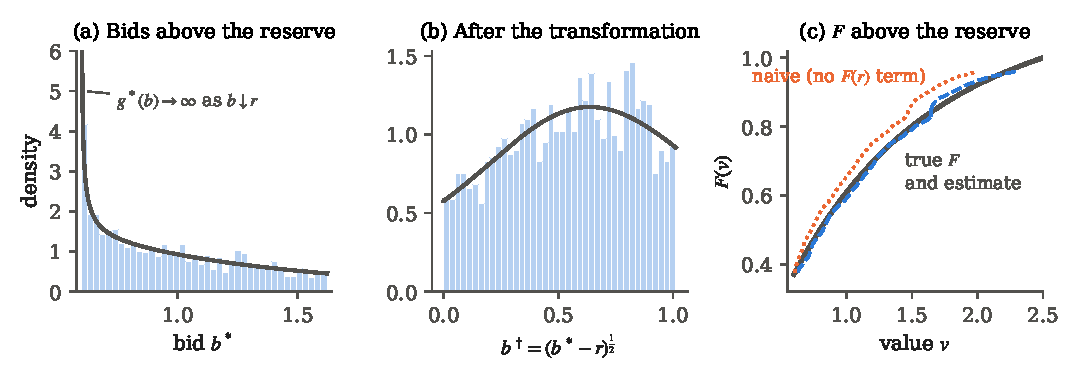
\includegraphics[width=\textwidth]{figures/ch15/gpv_reserve.pdf}
\caption{A binding reserve price. $T=500$ auctions with $N=5$ potential bidders, values lognormal$(0,1)$ truncated to $[0.055,2.5]$, reserve price $r=0.6$ with $F(r)=0.370$. Panel (a): histogram of the 1,627 actual bids and the true density $g^*$, which diverges at $r$. Panel (b): the transformed bids $(b^*-r)^{\frac12}$ have a bounded density. Panel (c): true $F$ above $r$ (solid), the estimate based on \eqref{eq:15-gpv-reserve-dagger} with $\hat N=5$ and $\hat F(r)=0.349$ (dashed), and a naive estimate that drops the term in $F(r)$ (dotted). Our simulation (seed 15404).}\label{fig:15-gpv-reserve}
\end{figure}

\Cref{fig:15-gpv-reserve} applies the procedure to simulated data. With $N=5$ and $r=0.6$, the expected number of actual bidders is $5(1-0.370)=3.15$. In the sample, $\hat N=5$ and $\hat F(r)=1-\frac{3.254}{5}=0.349$. The design has no covariates, and the estimates of $G^\dagger$ and $g^\dagger$ pool all 1,627 actual bids. The one auction of the 500 without a bid therefore enters only $\hat F(r)$. Among bids that survive trimming, the mean absolute error of the pseudo-values is 0.025 with the full formula and 0.151 for the naive formula without the term in $F(r)$. For values within 0.3 of the reserve, the naive pseudo-values are too low by 0.078 on average. The missing term is the markdown that comes from competing against potential bidders who stay out.

\casehead{Affiliated values and observed participation} \Citet[Section 6.3.1]{AtheyHaile2007} extend these results to affiliated private values when bidders do not know the set of actual bidders. With all bids, bidder identities and the reserve price, the joint distribution of the actual bidders' values above $r$ is identified (their Theorem 6.4). Each marginal $F_i$ is identified above $r$ when the set of potential bidders is observed (their Theorem 6.5). \Cref{sec:15-entry-reserve} states these results and the inversion behind them. Exogenous variation in reserve prices would trace out more of $F$, as GPV note. Estimators that combine auctions with different reserve prices to recover $F$ below the observed reserves had not been developed when Athey and Haile wrote their survey \citep[Section 6.3.1]{AtheyHaile2007}. \Cref{sec:15-uh} discusses the opposite case, in which the reserve price carries information about the object.

\subsection{Incomplete bid data and Dutch auctions}\label{sec:15-gpv-winbid}

Many data sets record only the winning bid. In a Dutch auction the clock stops at the first bid, so only the transaction price exists. The Dutch auction is strategically equivalent to the first-price auction (\cref{prop:14-dutch-fpa}). In other settings the auctioneer records only the winner. With independent private values, the winning bid suffices.

\begin{proposition}[\citealp{AtheyHaile2002}, Theorem 6(i), and \citealp{AtheyHaile2007}, Theorem 3.2 and Corollary 3.1]\label{prop:15-winbid}
In a first-price or Dutch auction with independent private values, suppose the transaction price and the number of bidders are observed. If bidders are asymmetric, suppose also that the set of bidders and the identity of the winner are observed. Then the value distribution of every bidder is identified.
\end{proposition}

\begin{proof}
\emph{Symmetric bidders.} Let $G_{(n:n)}$ denote the distribution of the winning bid $B^{(n:n)}$, with density $g_{(n:n)}$. Bids are i.i.d.\ with distribution $G$, so $G_{(n:n)}(b)=G(b)^n$ and
\begin{equation}\label{eq:15-winbid-G}
G(b)=G_{(n:n)}(b)^{\frac1n}.
\end{equation}
Hence the winning bid identifies the distribution of a single bid, and \cref{thm:15-gpv-ident} applies. To write the inverse bid function directly in terms of the winning bid, differentiate: $g_{(n:n)}(b)=nG(b)^{n-1}g(b)$. Then
\[
\frac{G_{(n:n)}(b)}{g_{(n:n)}(b)}=\frac{G(b)^n}{nG(b)^{n-1}g(b)}=\frac{G(b)}{ng(b)}=\frac{n-1}{n}\cdot\frac{G(b)}{(n-1)g(b)},
\]
which is equation (3.7) of \citet{AtheyHaile2007}. Substituting into \eqref{eq:15-gpv-xi},
\begin{equation}\label{eq:15-winbid-xi}
\xi(b)=b+\frac{n}{n-1}\,\frac{G_{(n:n)}(b)}{g_{(n:n)}(b)}.
\end{equation}
This observation is due to \citet{GuerrePerrigneVuong1995}.

\emph{Asymmetric bidders.} Let $G_i$ denote the distribution of bidder $i$'s bid, and let $G^w_i(b)=\Pr(B_i\le b,\ B_i\ge B_j\text{ for all }j)$ be the probability that $i$ wins with a bid of at most $b$. It is observable when the winner's identity is recorded. By independence,
\[
G^w_i(b)=\int_{\underline b}^b\prod_{j\neq i}G_j(s)\,dG_i(s).
\]
Summing over bidders, $\sum_jG^w_j(s)=\Pr(\max_jB_j\le s)=\prod_jG_j(s)$, the distribution of the winning bid. Therefore
\[
\frac{dG^w_i(s)}{\sum_jG^w_j(s)}=\frac{\prod_{j\neq i}G_j(s)\,dG_i(s)}{\prod_jG_j(s)}=\frac{dG_i(s)}{G_i(s)}=d\ln G_i(s).
\]
Integrating from $b$ to $\bar b$ and using $G_i(\bar b)=1$ gives
\begin{equation}\label{eq:15-berman}
G_i(b)=\exp\Big\{-\int_b^{\bar b}\Big(\sum_{j=1}^nG^w_j(s)\Big)^{-1}dG^w_i(s)\Big\}.
\end{equation}
This is the competing-risks formula of \citet{Berman1963}, adapted to auctions by \citet{AtheyHaile2002}. The right side is observable, so each $G_i$ is identified. The marginals $G_j$ determine the distribution of each bidder's highest rival bid, $G_{M_i}=\prod_{j\neq i}G_j$. The asymmetric first-order condition \eqref{eq:14-asym-foc}, rearranged as $v_i=b+\big[\sum_{j\neq i}\frac{g_j(b)}{G_j(b)}\big]^{-1}$, then gives each inverse bid function and each $F_i$.
\end{proof}

The formula in \citet[eq.~(3.8)]{AtheyHaile2007} is printed with the integral running from $-\infty$ to $b$ and without the minus sign. The derivation above gives the form \eqref{eq:15-berman}. \Citet{BrendstrupPaarsch2003} propose estimating \eqref{eq:15-berman} by replacing $G^w_i$ with its empirical counterpart and $dG^w_i$ with a kernel estimate \citep[Section 3.3.1]{AtheyHaile2007}. Athey and Haile add that survival-analysis estimators such as the Kaplan-Meier or Nelson-Aalen estimators could be adapted.

\casehead{Estimation with symmetric bidders} With $T$ winning bids $B^w_t$, one estimates $G_{(n:n)}$ by the empirical distribution and $g_{(n:n)}$ by a kernel estimator. Equation \eqref{eq:15-winbid-xi} then gives the estimated winner's value $\hat V^{(n:n)}_t=\hat\xi(B^w_t)$, after trimming as in \eqref{eq:15-gpv-trim}. The winners' values have distribution $F^n$, so $\hat F(v)=\big[\frac1T\sum_t\indic(\hat V^{(n:n)}_t\le v)\big]^{\frac1n}$.

\casehead{The cost of observing only the winner} The data contain one bid per auction instead of $n$, and the inversion through the $n$-th root loses precision in the lower tail. To see how much, ignore first-step error and suppose the winners' values were observed. Let $H=F^n$ and let $\hat H$ be the empirical distribution of the $T$ winners' values, with variance $\frac{H(1-H)}{T}$. Since $\frac{dF}{dH}=\frac1nH^{\frac1n-1}=\frac1nF^{1-n}$, the delta method gives
\[
\Var\big(\hat F(v)\big)\approx\frac{1}{n^2}F^{2-2n}\,\frac{F^n(1-F^n)}{T}=\frac{F^{2-n}(1-F^n)}{n^2T}.
\]
With all $nT$ values observed, the variance of the empirical distribution is $\frac{F(1-F)}{nT}$. The ratio of the two variances is
\[
\frac{F^{2-n}(1-F^n)}{n^2T}\cdot\frac{nT}{F(1-F)}=\frac{1-F^n}{nF^{n-1}(1-F)}=\frac{1+F+\dots+F^{n-1}}{nF^{n-1}}.
\]
It equals one at the top of the support and grows without bound as $F\to0$. With $n=5$ at the median of $F$, the ratio is $\frac{1.9375}{0.3125}=6.2$. This is our calculation. The winning bid identifies $F$, but low values are rarely revealed by winners, so the lower tail is estimated poorly.

\casehead{An unknown number of bidders} In some Dutch auctions only the transaction price is recorded, and the number of bidders is unknown. Then $F$ is not identified nonparametrically \citep[Section 3.3.1]{AtheyHaile2007}. For any candidate $n'$, the distribution $G_{(n:n)}^{\frac{1}{n'}}$ is a valid bid distribution, and $n'$ bidders bidding i.i.d.\ from it generate the same winning-bid distribution. Each $n'$ for which the implied inverse bid function is increasing yields a different $F$. \Citet{LaffontOssardVuong1995} instead estimate $n$ within a parametric model (\cref{sec:15-direct}).

\casehead{Covariates and testability} \Citet[Theorem 6]{AtheyHaile2002} extend the result in three directions. If $V_i=g_i(A_i,W_0)$ with $W_0$ observed by bidders and the econometrician and $A_1,\dots,A_n$ independent given $W_0$, then each $F_i(\cdot\mid w_0)$ is identified, because part (i) applies for each fixed $w_0$. If $V_i=g_0(W_0)+A_i$ with the $A_i$ mutually independent and independent of $W_0$, then each $F_{A_i}$ and $g_0$ are identified up to location. Finally, the models are testable. With symmetric bidders, observing more than one bid per auction, or exogenous variation in $n$, gives two estimates of $G$ from \eqref{eq:15-winbid-G} that must agree. With asymmetric bidders, observing the second-highest bid or exogenous variation in $n$ plays the same role \citep[Theorem 6(iv)--(v)]{AtheyHaile2002}.

\subsection{Specification testing in first-price auctions}\label{sec:15-gpv-tests}

\Cref{thm:15-gpv-ident} lists the restrictions that the SIPV model places on bids. \Citet[Section 5.1]{AtheyHaile2007} characterize the restrictions in the broader affiliated private values (APV) model of \cref{sec:15-apv}. Write $\xi_i(b;\mathcal N)=b+\frac{G_{M_i\mid B_i}(b\mid b;\mathcal N)}{g_{M_i\mid B_i}(b\mid b;\mathcal N)}$ for bidder $i$'s inverse bid function when the set of bidders is $\mathcal N$. Here $M_i$ is the highest rival bid and $G_{M_i\mid B_i}$ its distribution conditional on $i$'s bid, as in \eqref{eq:15-lpv-foc}. Let $[\underline b_i,\bar b_i]$ be the support of $B_i$.

\begin{theorem}[\citealp{AtheyHaile2007}, Theorem 5.2]\label{thm:15-ah-rational}
Consider the APV first-price auction with a fixed set of bidders $\mathcal N$. Assume the joint density of values is continuously differentiable, and that either (i) values are mutually independent or (ii) bidders are symmetric. A joint distribution of bids $\mathbf G$ is rationalized by equilibrium bidding if and only if:
\begin{itemize}
\item[(a)] The bids $(B_1,\dots,B_n)$ are affiliated. They are independent in case (i) and exchangeable in case (ii).
\item[(b)] Each $\xi_i(\cdot;\mathcal N)$ is differentiable and strictly increasing on the support of $B_i$.
\item[(c)] The distribution $\mathbf G\big(\xi_1^{-1}(u_1;\mathcal N),\dots,\xi_n^{-1}(u_n;\mathcal N)\big)$ is absolutely continuous in $\bm u$. Its density is positive and continuously differentiable on the product of the supports of $\xi_i(B_i;\mathcal N)$ and zero elsewhere.
\item[(d)] $\xi_i(\underline b;\mathcal N)=\underline b$ for all $i$.
\item[(e)] $\xi_i(\bar b_i;\mathcal N)=\xi_j(\bar b_j;\mathcal N)$ for all $i,j$.
\item[(f)] The support of $B_i$ is convex, compact, and the same for all $i$.
\end{itemize}
\end{theorem}

Without independence or symmetry, conditions of this type remain necessary but are not known to be sufficient. The equilibrium of the asymmetric APV model lacks a full characterization \citep[Theorem 5.1]{AtheyHaile2007}. Sufficiency in \cref{thm:15-ah-rational} uses the argument of Step 4 in the proof of \cref{thm:15-gpv-ident}. Under independence or symmetry, payoffs satisfy single crossing. Local optimality of each bid together with monotone strategies then implies global optimality. Athey and Haile stress why such a result matters. Without it, nothing guarantees that a bid $b$ is a best response for the value $\xi_i(b)$ that the first-order condition assigns to it. Verifying the conditions is the analog of verifying second-order conditions \citep[Section 5.1]{AtheyHaile2007}. For SIPV, the conditions reduce to (C1)--(C2) of \cref{thm:15-gpv-ident}.

Each condition suggests a test. We describe the main ones, following \citet[Sections 5.2--5.5]{AtheyHaile2007}.

\casehead{Monotonicity of the inverse bid function} Condition (C2), or (b), says that $\hat\xi$ should be increasing. GPV propose this as a test of equilibrium bidding and note that it requires estimating $\xi$ under a monotonicity constraint \citep[p.~552]{GuerrePerrigneVuong2000}. No formal test had been developed by the time of the Athey-Haile survey. Standard tests of monotone regression do not apply directly, because the realizations $\xi_i(B_i)$ are themselves estimates. Applications typically find few violations \citep{HendricksPinksePorter2003,HaileHongShum2003}. Two caveats apply. First, a rejection does not reveal which assumption failed: unobserved heterogeneity, risk aversion, or non-equilibrium play could each cause it. Second, no test of monotonicity is consistent against all violations of the model, since some misspecified models still produce an increasing $\xi$.

\casehead{The boundary condition} Condition (e) says that all bidders' inverse bid functions meet at the top of the bid support, since all bidders share the upper bound of values. In the asymmetric IPV model, $G_{M_i}(\bar b)=1$, so $\xi_i(\bar b)=\bar b+\frac{1}{g_{M_i}(\bar b)}$, and (e) becomes
\begin{equation}\label{eq:15-boundary-test}
g_{M_i}(\bar b)=g_{M_j}(\bar b)\qquad\text{for all }i,j,
\end{equation}
which is equation (5.1) of \citet{AtheyHaile2007}. The densities of the highest rival bid must agree at the top. \Cref{sec:15-apv-asym} works through an example of Athey and Haile in which the condition fails because the value supports of the two bidders have different upper bounds, which the maintained model excludes.

\casehead{Multi-sample tests with exogenous variation in $n$} If the number of bidders varies exogenously, the value distribution estimated from $n$-bidder auctions must equal the one estimated from $n'$-bidder auctions. Under IPV, the inverse bid functions $\xi(\cdot;G_n,n)$ differ across $n$, because bidding becomes more aggressive as $n$ rises (\cref{prop:14-fpa-n}). The implied value distributions must nevertheless coincide. Testing equality of distributions is standard when the data are observed. Here the values are estimated in a first nonparametric step, which complicates the asymptotic theory. \Citet{HaileHongShum2003} develop formal tests of this kind. They use them to test private against common values, which \cref{sec:15-cv} takes up.

\casehead{Multiple order statistics} In IPV models, any single order statistic of bids identifies $F$, together with $n$. When two order statistics are recorded, for example the two highest bids, the two implied estimates of $F$ must agree up to sampling error. This test needs no variation in $n$ \citep[Section 5.4]{AtheyHaile2007}.

\casehead{Direct tests of independence and exchangeability} Condition (C1) can be tested directly when all bids are observed. Exchangeability can be tested with the bootstrap distance tests of \citet{Romano1988,Romano1989}, which compare a multivariate distribution with its permutations. Equality of the marginal distributions of different bidders can be tested by Kolmogorov-Smirnov statistics. Independence can be tested by comparing the joint distribution of bids with the product of its marginals. GPV suggest the test of \citet{BlumKieferRosenblatt1961}, which \citet{CampoPerrigneVuong2003} later apply to offshore oil bids. With covariates, regression tests of conditional independence and exchangeability are natural. \Cref{sec:15-collusion} describes them in the form that \citet{BajariYe2003} use to look for collusion in highway procurement.

\citet[p.~2123]{AtheyHaile2002} add a warning. Monotonicity of $\xi$ holds under many natural alternatives to the IPV model, so the test most often used in early work has little power against affiliated or common values. The restrictions that come from comparing different order statistics or different numbers of bidders typically fail under those alternatives. They are the more informative tests.

\casehead{Assessment} GPV changed the econometrics of auctions. Before them, structural work required closed-form equilibria or simulation, and parametric assumptions carried an unclear part of the identification \citep[Section 3.1]{AtheyHaile2007}. After them, the first-order condition became a measurement device. The ingredients were a constructive identification result with sharp testable restrictions, an estimator that requires only kernel smoothing, and a proof that the estimator is rate-optimal. The same principle extends to affiliated values, asymmetric bidders, procurement with quality, binding reserve prices and dynamic bidding. It also inspired parametric two-step estimators that keep the inversion and add structure in one of the steps \citep[footnote 25]{GuerrePerrigneVuong2000}.

The approach has limits that later sections address. It maintains independent private values and risk neutrality, and it assumes that observed covariates capture all heterogeneity across auctions. Ignoring unobserved heterogeneity flattens the estimated inverse bid function and inflates estimated markups (\cref{sec:15-uh}). The second step pools across $n$ only if participation is exogenous given covariates (\cref{sec:15-entry}). Each additional continuous covariate slows convergence, and the boundary trimming discards the tails of $F$, which matter for reserve prices. No distribution theory for $\hat f$ was available. Bandwidth constants are set by rules of thumb, and data-driven choices had not been explored \citep[Section 3.2.1]{AtheyHaile2007}. Finally, the model needs all bids, or the winning bid with known $n$. When bidding takes place under richer information structures, bids reveal less, as \cref{sec:15-apv,sec:15-cv} show.

The rest of the chapter relaxes the maintained assumptions one at a time. \Cref{sec:15-apv} replaces independence with affiliation and symmetry with bidder classes, and the inversion runs through the distribution of the highest rival bid conditional on one's own bid. \Cref{sec:15-cv} asks what bids can reveal when values are common. \Cref{sec:15-uh} handles heterogeneity that bidders observe and the econometrician does not. \Cref{sec:15-entry} treats endogenous participation, dynamics and risk aversion. In each case the first step of the GPV estimator survives, and the work lies in finding the right conditioning set for the distribution of rival bids.
